
\section{Appendix}

\subsection{Filter Selection Timing Analysis}

We include the timing records of our filter selection. 
Both routines were run on NVIDIA GPU environment with the Brute Force run pruned to cosine similarity of .95 and able to utilize 8 GPUs. 
Conversely, the PCA algorithm used one GPU for calculation and 8 GPUs only for the augmented steps. 

\begin{table}[htbp]
    \begin{tabular}{llrrrrrr}
    \toprule
    &  & \multicolumn{2}{r}{Base Time (s)} & \multicolumn{2}{r}{Aug Time (s)} & \multicolumn{2}{r}{Total Time (s)} \\
    & Strategy & Brute Force & PCA & Brute Force & PCA & Brute Force & PCA \\
    $k_1$ & $k_2$ &  &  &  &  &  &  \\
    \midrule
    \multirow[t]{3}{*}{1} & 0 & 13.70 & 7.50 & 0.00 & 0.00 & 13.70 & 7.50 \\
    & 1 & 13.70 & 7.50 & 19.23 & 19.98 & 32.93 & 27.48 \\
    & 2 & 13.70 & 7.50 & 20.61 & 20.89 & 34.31 & 28.40 \\
    \cline{1-8}
    \multirow[t]{3}{*}{2} & 0 & 12.58 & 6.80 & 0.00 & 0.00 & 12.58 & 6.80 \\
    & 1 & 12.58 & 6.80 & 20.83 & 20.41 & 33.41 & 27.20 \\
    & 2 & 12.58 & 6.80 & 20.30 & 18.34 & 32.88 & 25.13 \\
    \cline{1-8}
    \multirow[t]{3}{*}{3} & 0 & 13.26 & 5.85 & 0.00 & 0.00 & 13.26 & 5.85 \\
    & 1 & 13.26 & 5.85 & 18.26 & 20.08 & 31.52 & 25.93 \\
    & 2 & 13.26 & 5.85 & 21.61 & 19.95 & 34.87 & 25.80 \\
    \cline{1-8}
    \multirow[t]{3}{*}{4} & 0 & 16.03 & 7.55 & 0.00 & 0.00 & 16.03 & 7.55 \\
    & 1 & 16.03 & 7.55 & 18.69 & 19.39 & 34.71 & 26.94 \\
    & 2 & 16.03 & 7.55 & 19.11 & 18.75 & 35.13 & 26.30 \\
    \cline{1-8}
    \multirow[t]{3}{*}{5} & 0 & 18.88 & 5.80 & 0.00 & 0.00 & 18.88 & 5.80 \\
    & 1 & 18.88 & 5.80 & 19.69 & 19.23 & 38.57 & 25.03 \\
    & 2 & 18.88 & 5.80 & 19.61 & 18.86 & 38.49 & 24.65 \\
    \cline{1-8}
    \multirow[t]{3}{*}{6} & 0 & 33.33 & 6.04 & 0.00 & 0.00 & 33.33 & 6.04 \\
    & 1 & 33.33 & 6.04 & 17.74 & 18.10 & 51.07 & 24.14 \\
    & 2 & 33.33 & 6.04 & 18.54 & 20.12 & 51.87 & 26.15 \\
    \cline{1-8}
    \multirow[t]{3}{*}{7} & 0 & 81.34 & 6.26 & 0.00 & 0.00 & 81.34 & 6.26 \\
    & 1 & 81.34 & 6.26 & 19.17 & 19.45 & 100.51 & 25.71 \\
    & 2 & 81.34 & 6.26 & 19.11 & 19.72 & 100.45 & 25.98 \\
    \cline{1-8}
    \multirow[t]{3}{*}{8} & 0 & 190.31 & 6.55 & 0.00 & 0.00 & 190.31 & 6.55 \\
    & 1 & 190.31 & 6.55 & 20.31 & 20.26 & 210.62 & 26.81 \\
    & 2 & 190.31 & 6.55 & 20.17 & 20.80 & 210.49 & 27.35 \\
    \cline{1-8}
    \bottomrule
    \end{tabular}
    \caption{Timing Comparison: PCA vs. Brute Force, up to $k_1=8$, $k_2=2$}
    \label{tab:timing_comparison}

\end{table}
\newpage
We also include the full loss and $\dE$ results. 
Note that 'Brute Force with Augmentation' considers additional filters to only the top result at $k_1$, and hence can have worse MSE than the PCA solution, which maximizes for orthogonality among filters. 

\begin{table}[htbp]
    \centering
    \begin{tabular}{llrrrr}
    \toprule
     &  & \multicolumn{2}{r}{Best MSE} & \multicolumn{2}{r}{Best $\Delta E$} \\
     & Strategy & Brute Force & PCA & Brute Force & PCA \\
    $k_1$ & $k_2$ &  &  &  &  \\
    \midrule
    \multirow[t]{3}{*}{1} & 0 & 0.1904 & 0.2003 & 20.8603 & 17.7365 \\
      & 1 & 0.1432 & 0.0500 & 12.7010 & 12.6795 \\
      & 2 & 0.0263 & 0.0205 & 7.9875 & 4.6905 \\
    \cline{1-6}
    \multirow[t]{3}{*}{2} & 0 & 0.0489 & 0.0791 & 13.1686 & 13.5027 \\
      & 1 & 0.0392 & 0.0272 & 9.8836 & 6.9481 \\
      & 2 & 0.0188 & 0.0117 & 1.1743 & 1.8973 \\
    \cline{1-6}
    \multirow[t]{3}{*}{3} & 0 & 0.0219 & 0.0457 & 5.4475 & 2.8156 \\
      & 1 & 0.0220 & 0.0117 & 5.3174 & 1.8973 \\
      & 2 & 0.0089 & 0.0037 & 1.5786 & 0.5551 \\
    \cline{1-6}
    \multirow[t]{3}{*}{4} & 0 & 0.0063 & 0.0318 & 1.9277 & 1.6631 \\
      & 1 & 0.0229 & 0.0062 & 1.7381 & 0.9180 \\
      & 2 & 0.0033 & 0.0025 & 0.5718 & 0.3909 \\
    \cline{1-6}
    \multirow[t]{3}{*}{5} & 0 & 0.0034 & 0.0197 & 0.9064 & 0.5701 \\
      & 1 & 0.0108 & 0.0047 & 4.7085 & 0.7234 \\
      & 2 & 0.0021 & 0.0018 & 0.5258 & 0.4879 \\
    \cline{1-6}
    \multirow[t]{3}{*}{6} & 0 & 0.0021 & 0.0146 & 0.4550 & 0.6770 \\
      & 1 & 0.0033 & 0.0044 & 0.6592 & 0.6900 \\
      & 2 & 0.0018 & 0.0015 & 0.4961 & 0.4676 \\
    \cline{1-6}
    \bottomrule
    \end{tabular}
    \caption{Minimum MSE and $\Delta E$ Comparison: PCA vs. Brute Force, up to $k_1=6$, $k_2=2$}
    \label{tab:mse_deltae_comparison}
\end{table}

\subsection{Code Snippets}
We include code snippets from some of the algorithms outlined above and some of the infrastructure necessary for completing this research. 
The repository is available at this link: \href{https://github.com/kylefram/MultispectralCamera/tree/main}{https://github.com/kylefram/MultispectralCamera/tree/main}

\subsection{CAVE Dataset}

%%% TODO
%%% CHANGE TO GROUND TRUTH -> OTHERS instead of pairs with ground truths

We include images from the CAVE dataset, rendered under various $k \in \{2,3,4,8\}$ values. 
We consider the set of simulations including an IR-cut filter, and filters selected with the brute force methodology, having $k_2=0$.
Because the $k=8$ solution takes some time to brute force, we use a cosine similarity function to prune the filters to a set of 45, which reduces reconstruction quality and increases the differences in $\dE$ across renders. 

\begin{figure}[H]
\centering
\begin{subfigure}{.49\linewidth}
    \centering
    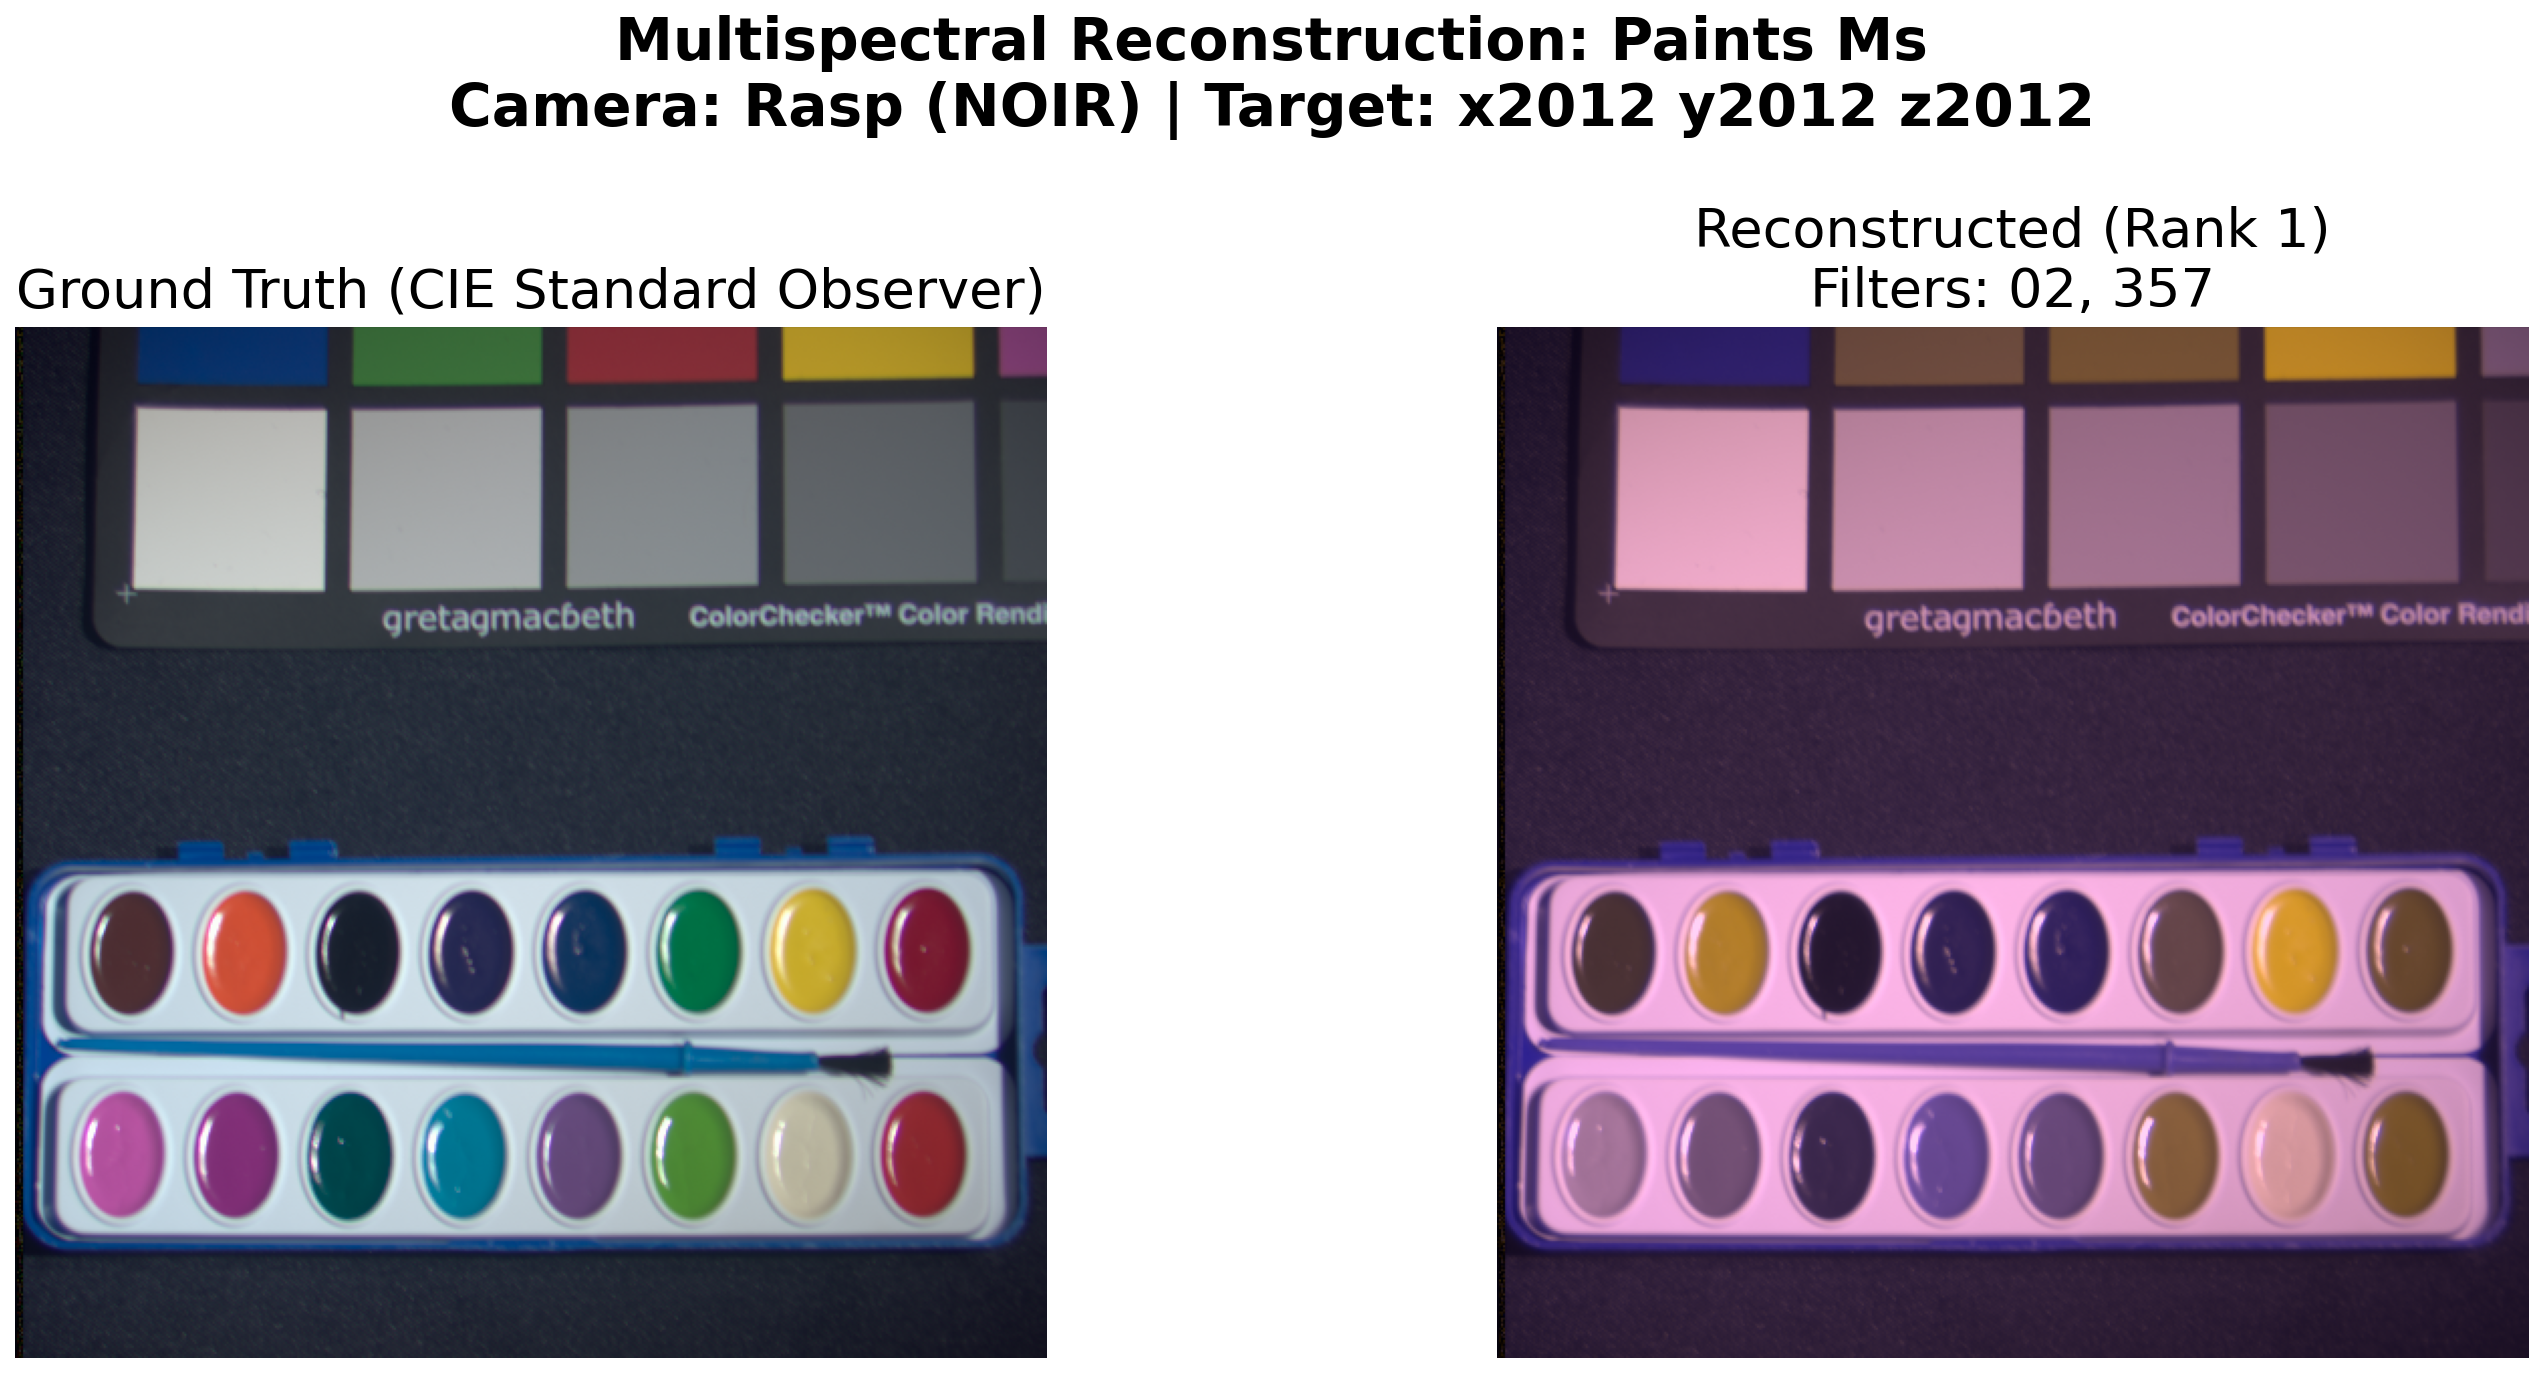
\includegraphics[width=\linewidth]{media/cave_appendix/k2paints.png}
    \caption{$k=2$, $\dE$=13.17}
\end{subfigure}
\begin{subfigure}{.49\linewidth}
    \centering
    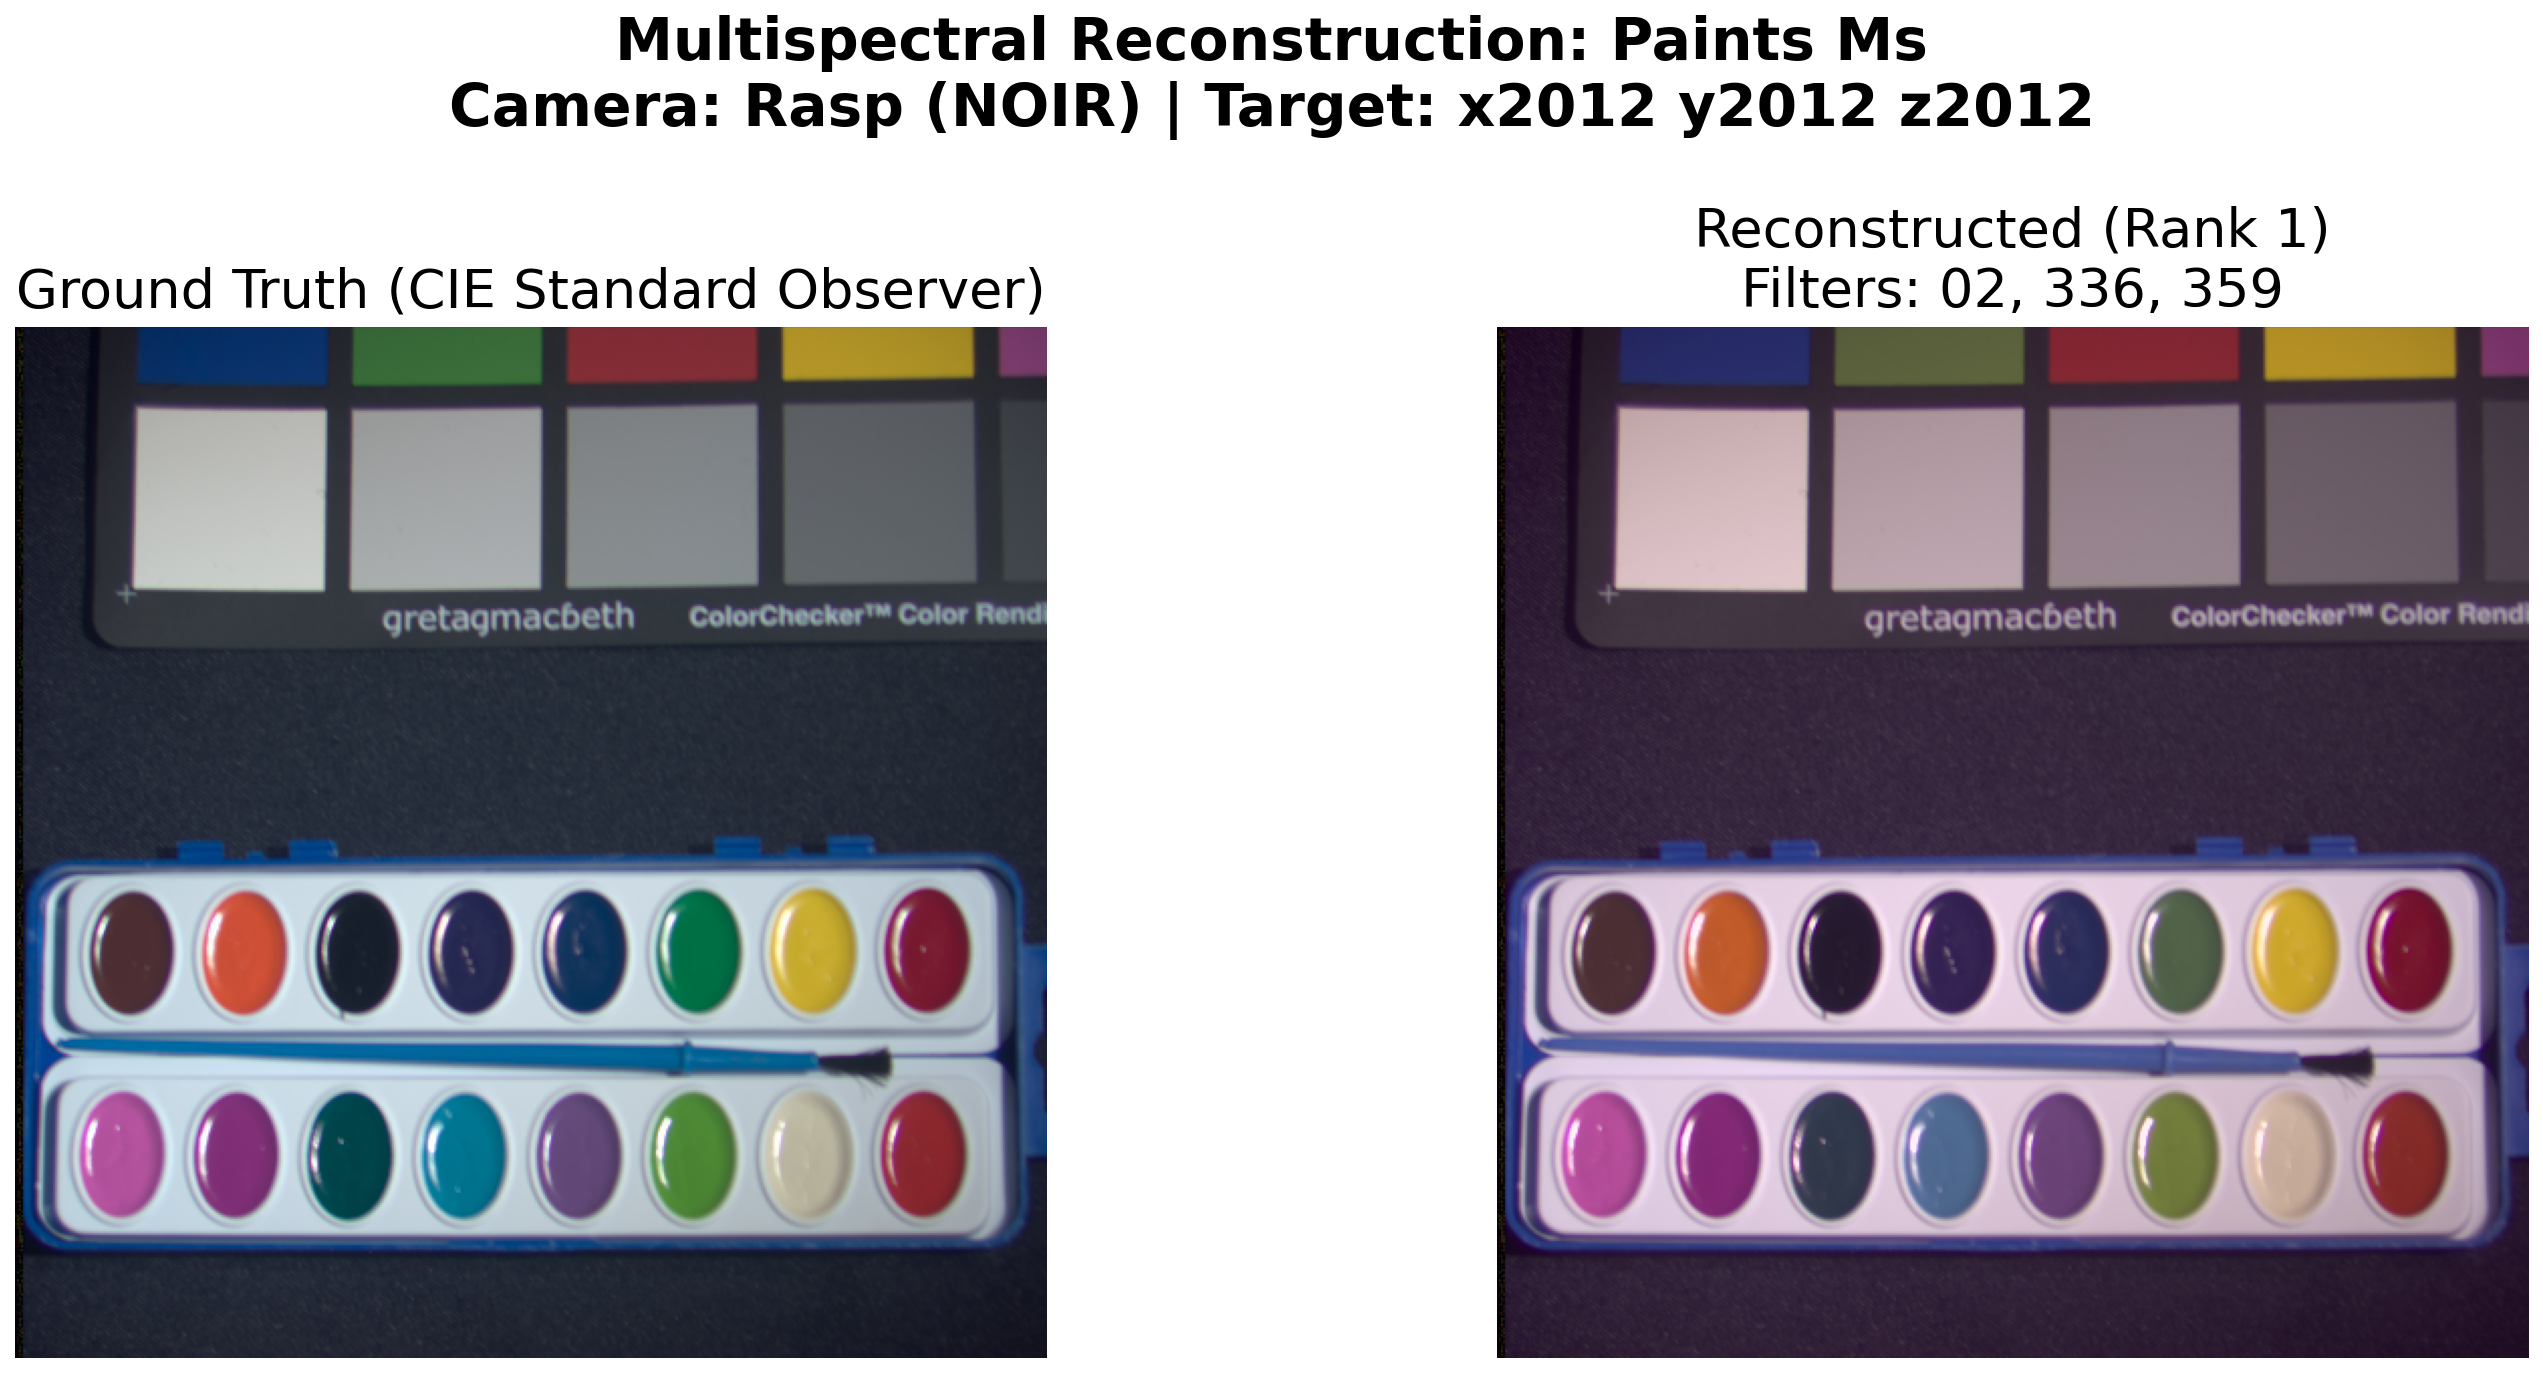
\includegraphics[width=\linewidth]{media/cave_appendix/k3paints.png}
    \caption{$k=3$, $\dE$=5.45}
\end{subfigure}
\begin{subfigure}{.49\linewidth}
    \centering
    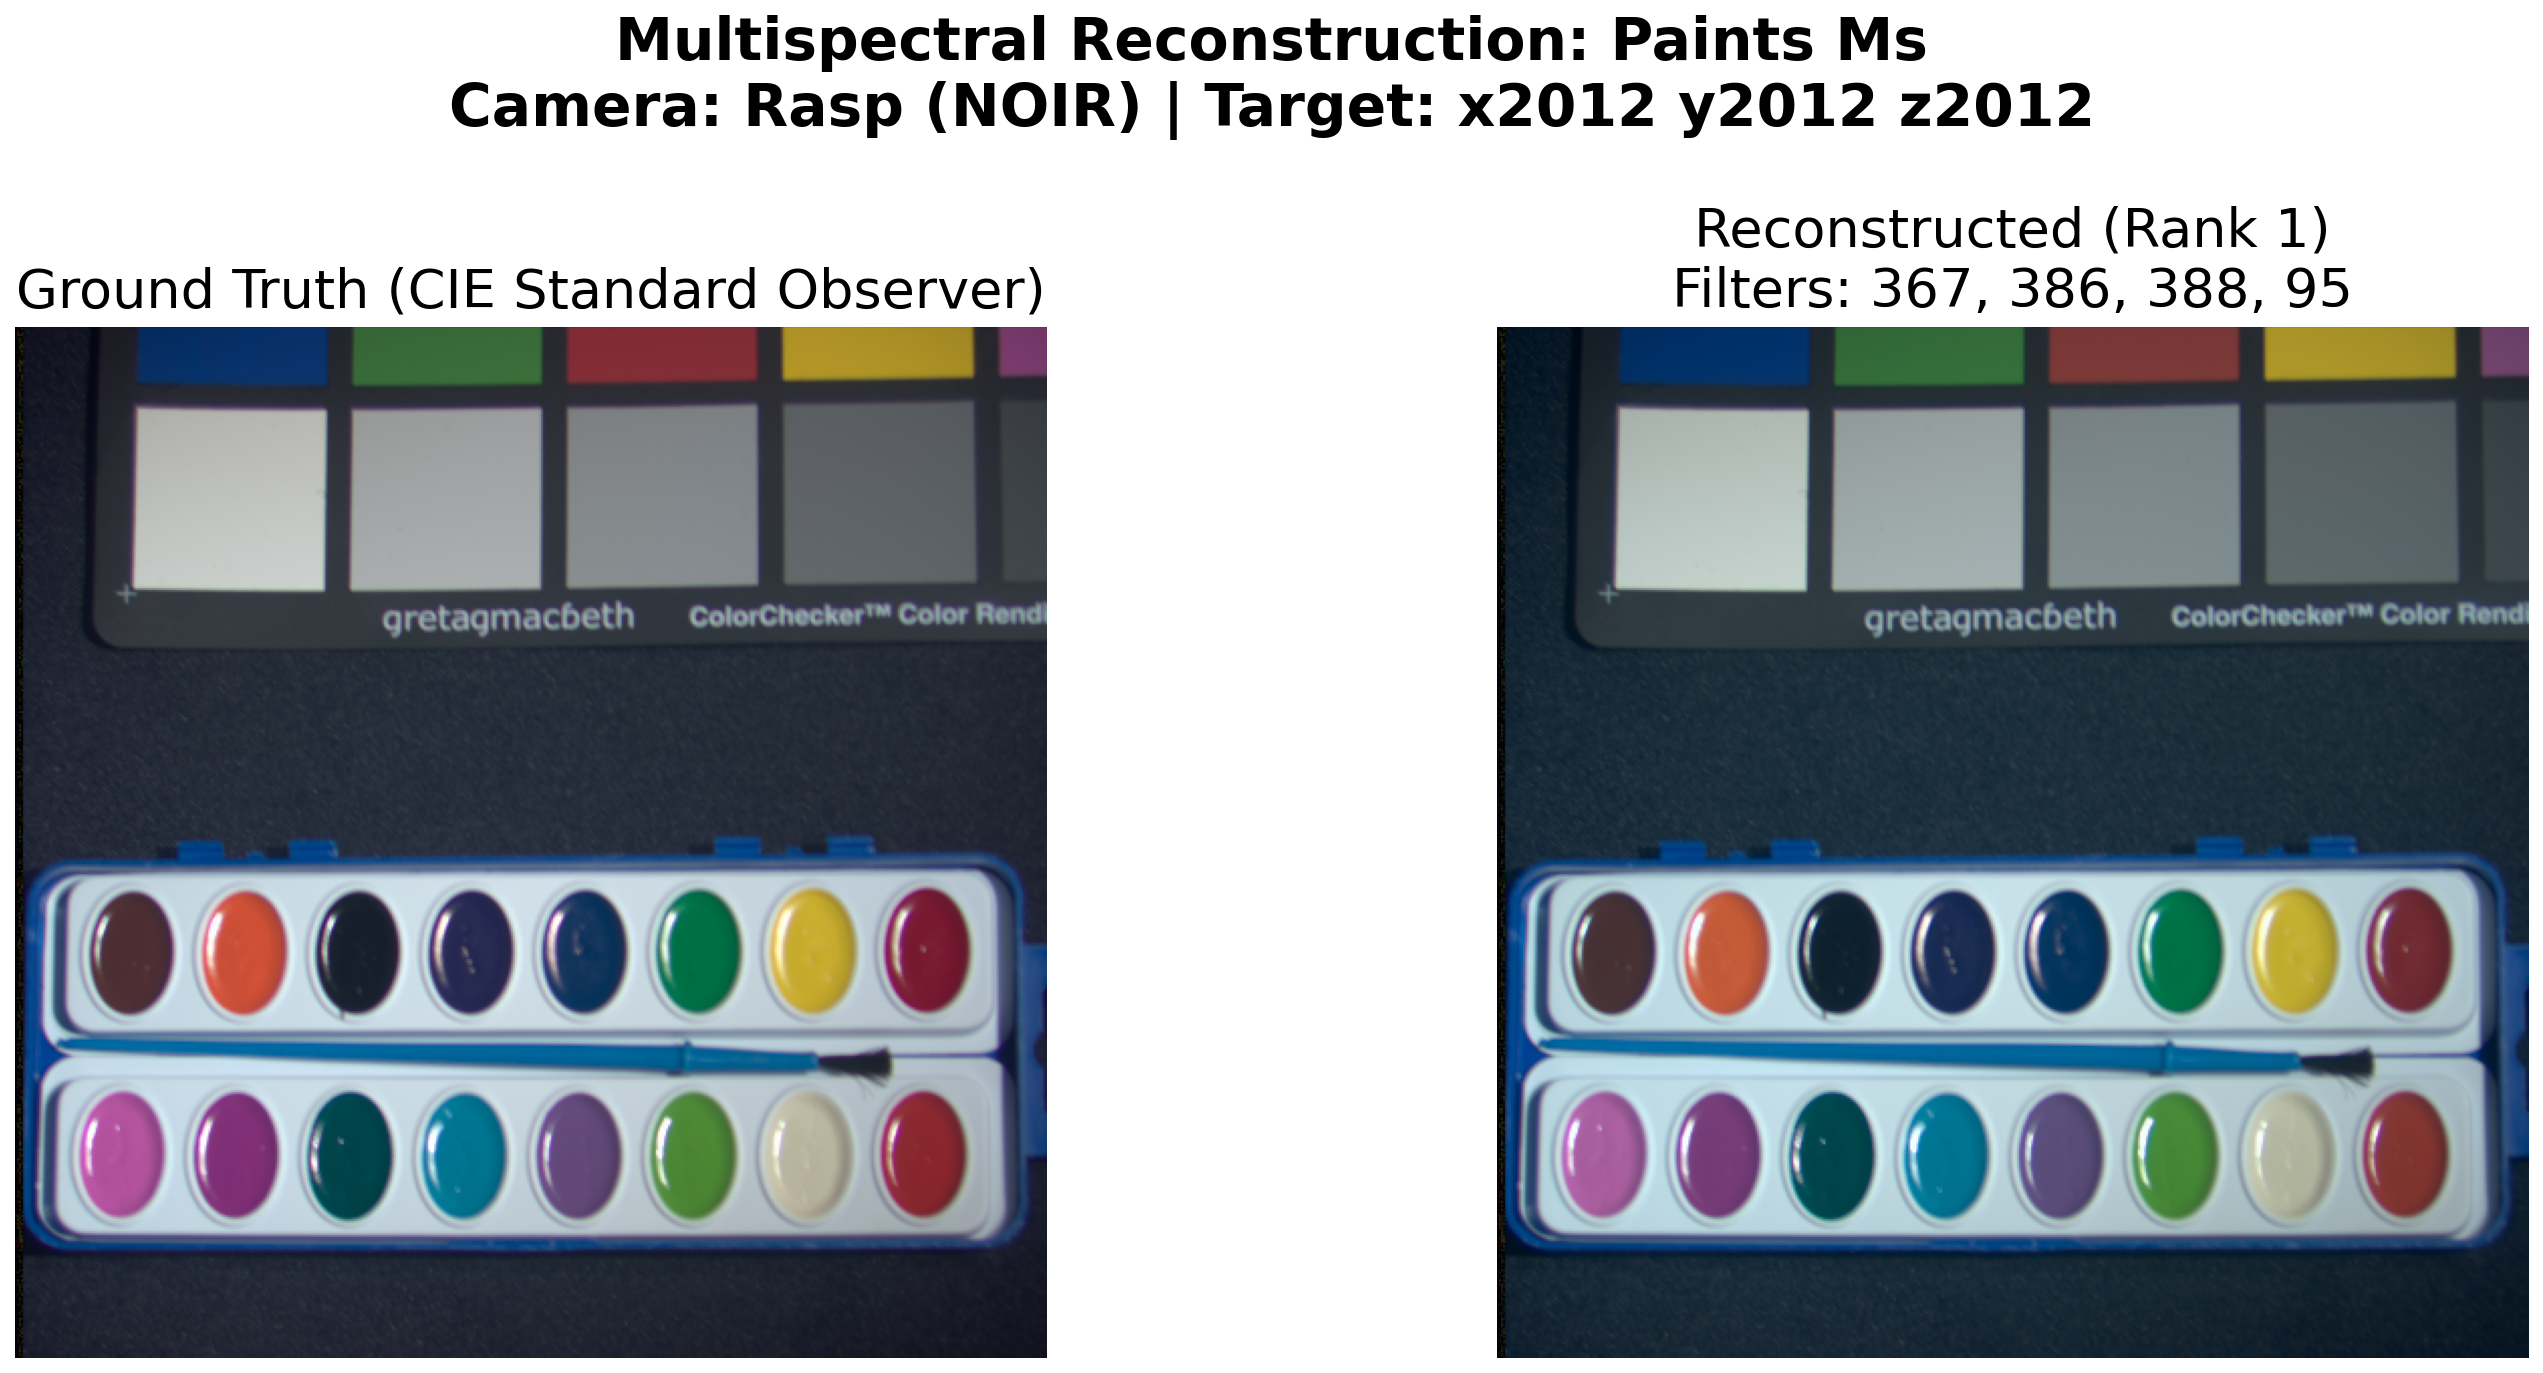
\includegraphics[width=\linewidth]{media/cave_appendix/k4paints.png}
    \caption{$k=4$, $\dE$=1.93}
\end{subfigure}
\begin{subfigure}{.49\linewidth}
    \centering
    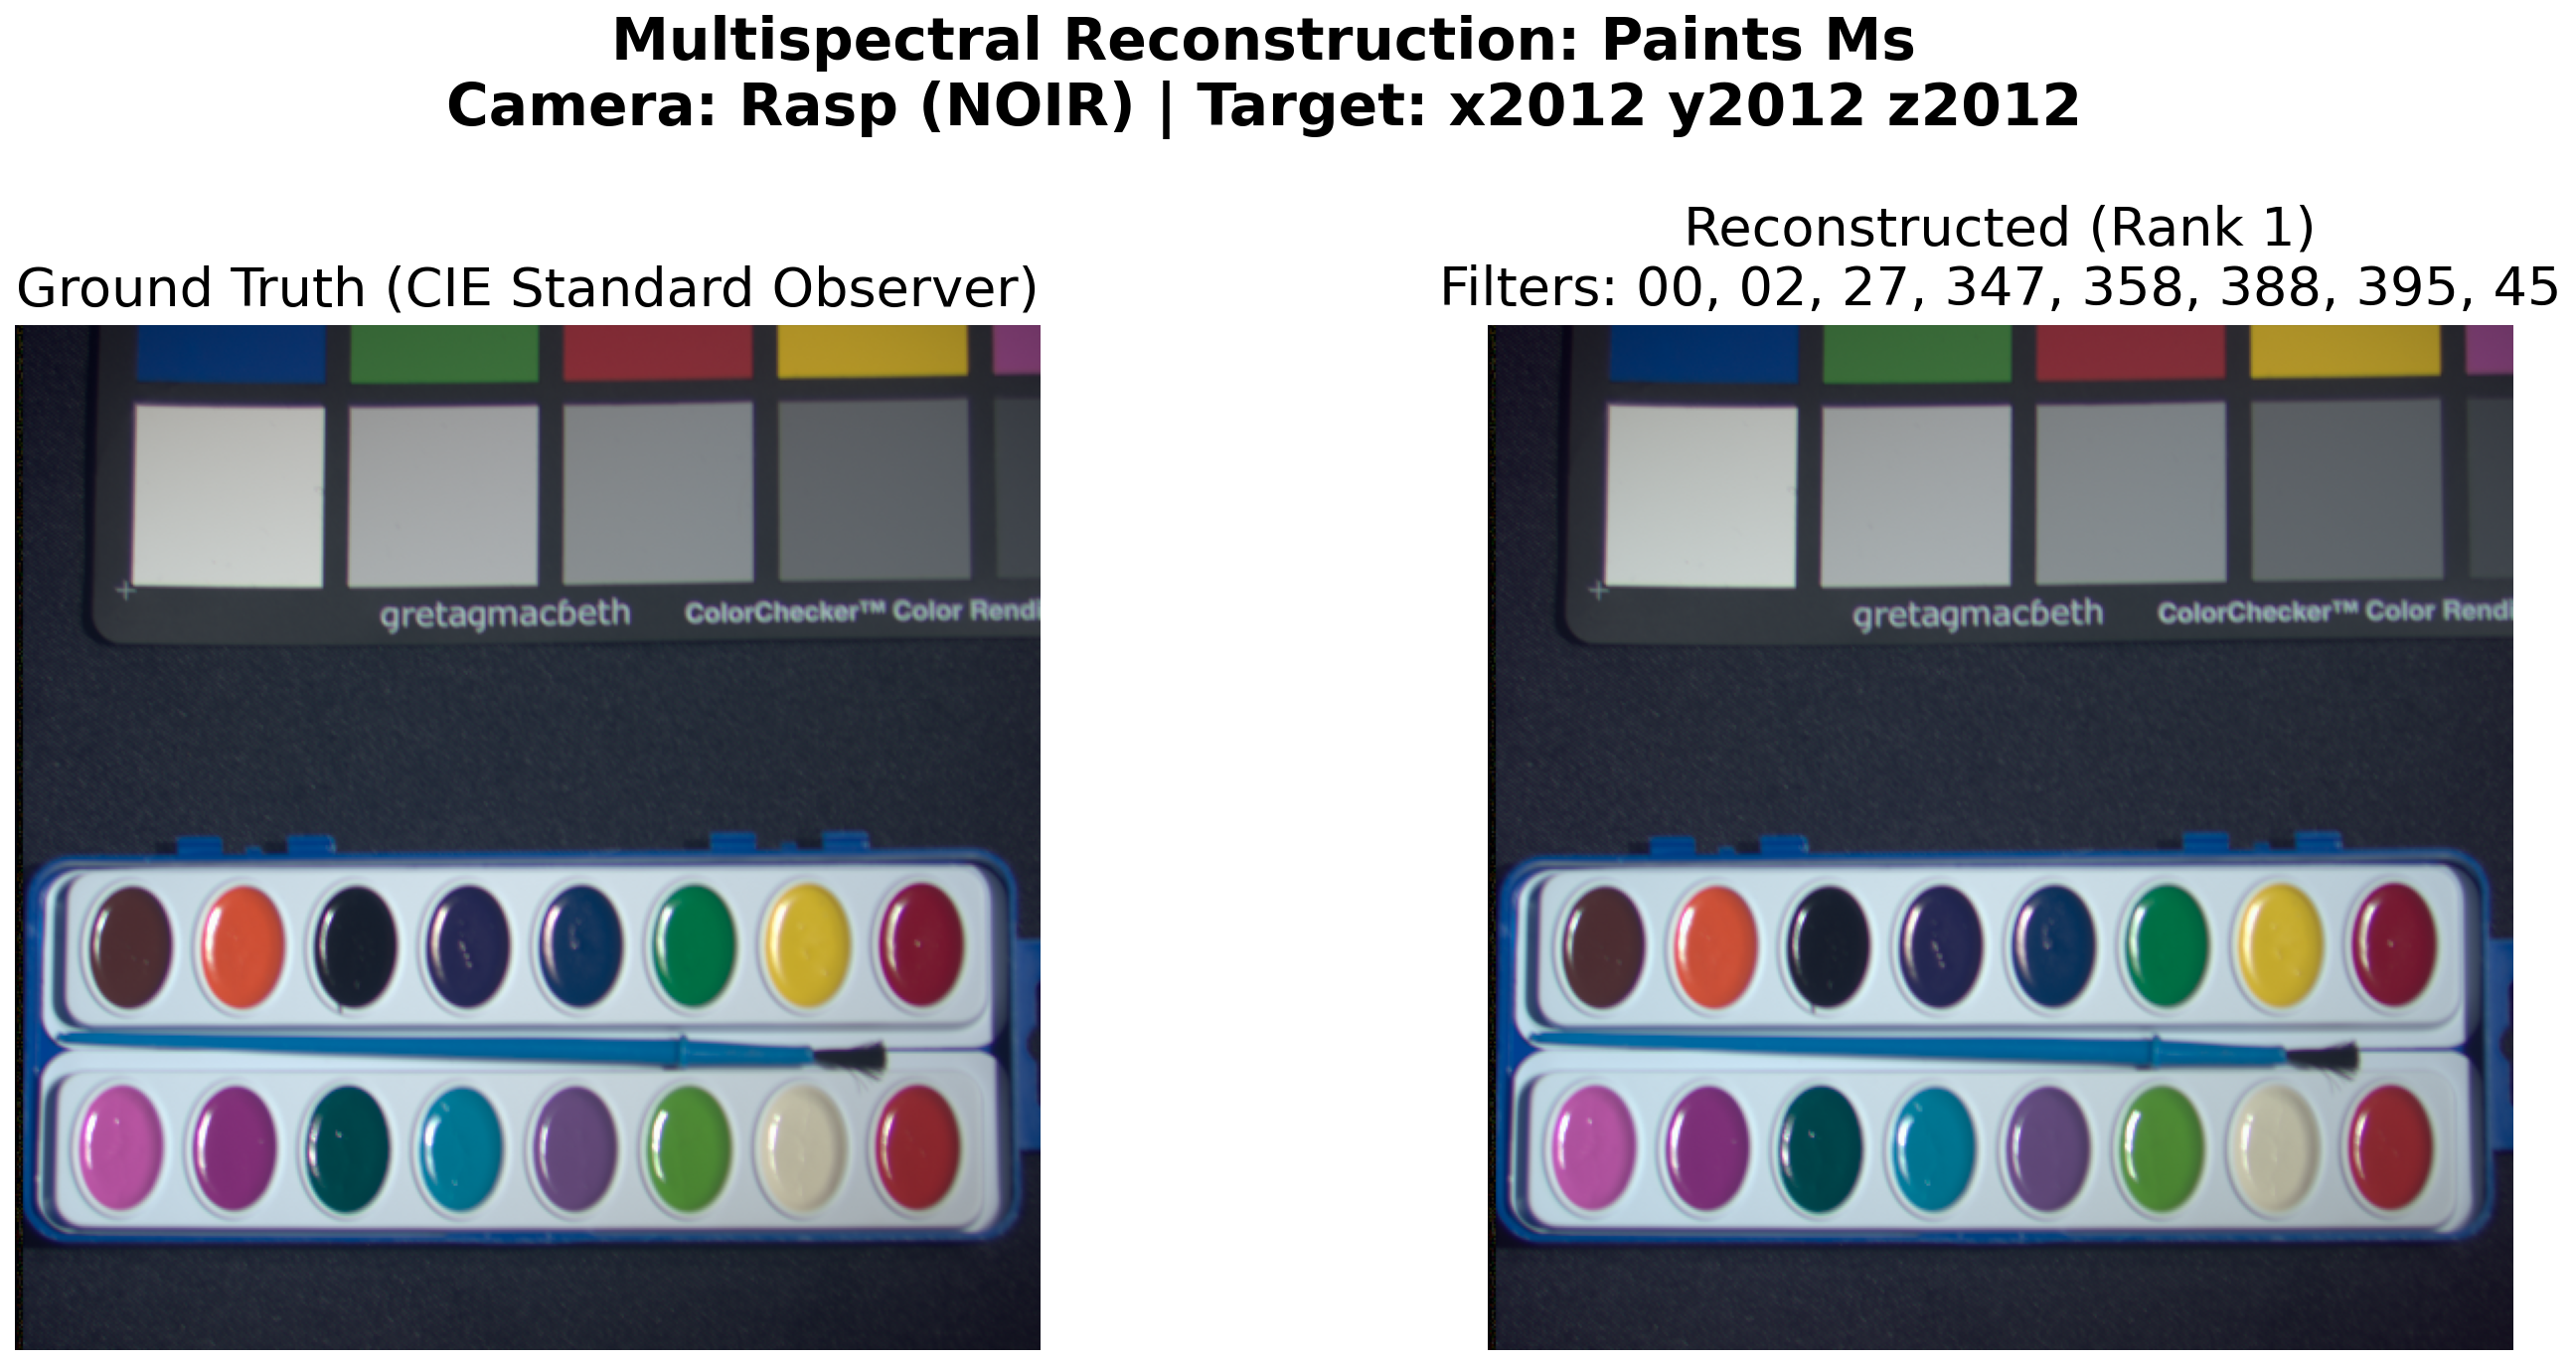
\includegraphics[width=\linewidth]{media/cave_appendix/k8paints.png}
    \caption{$k=8$, $\dE$=.61}
\end{subfigure}
\caption{CAVE Renders of Paints Multispectral Dataset, With Macbeth $\dE$}
\end{figure}

\begin{figure}[H]
\centering
\begin{subfigure}{.49\linewidth}
    \centering
    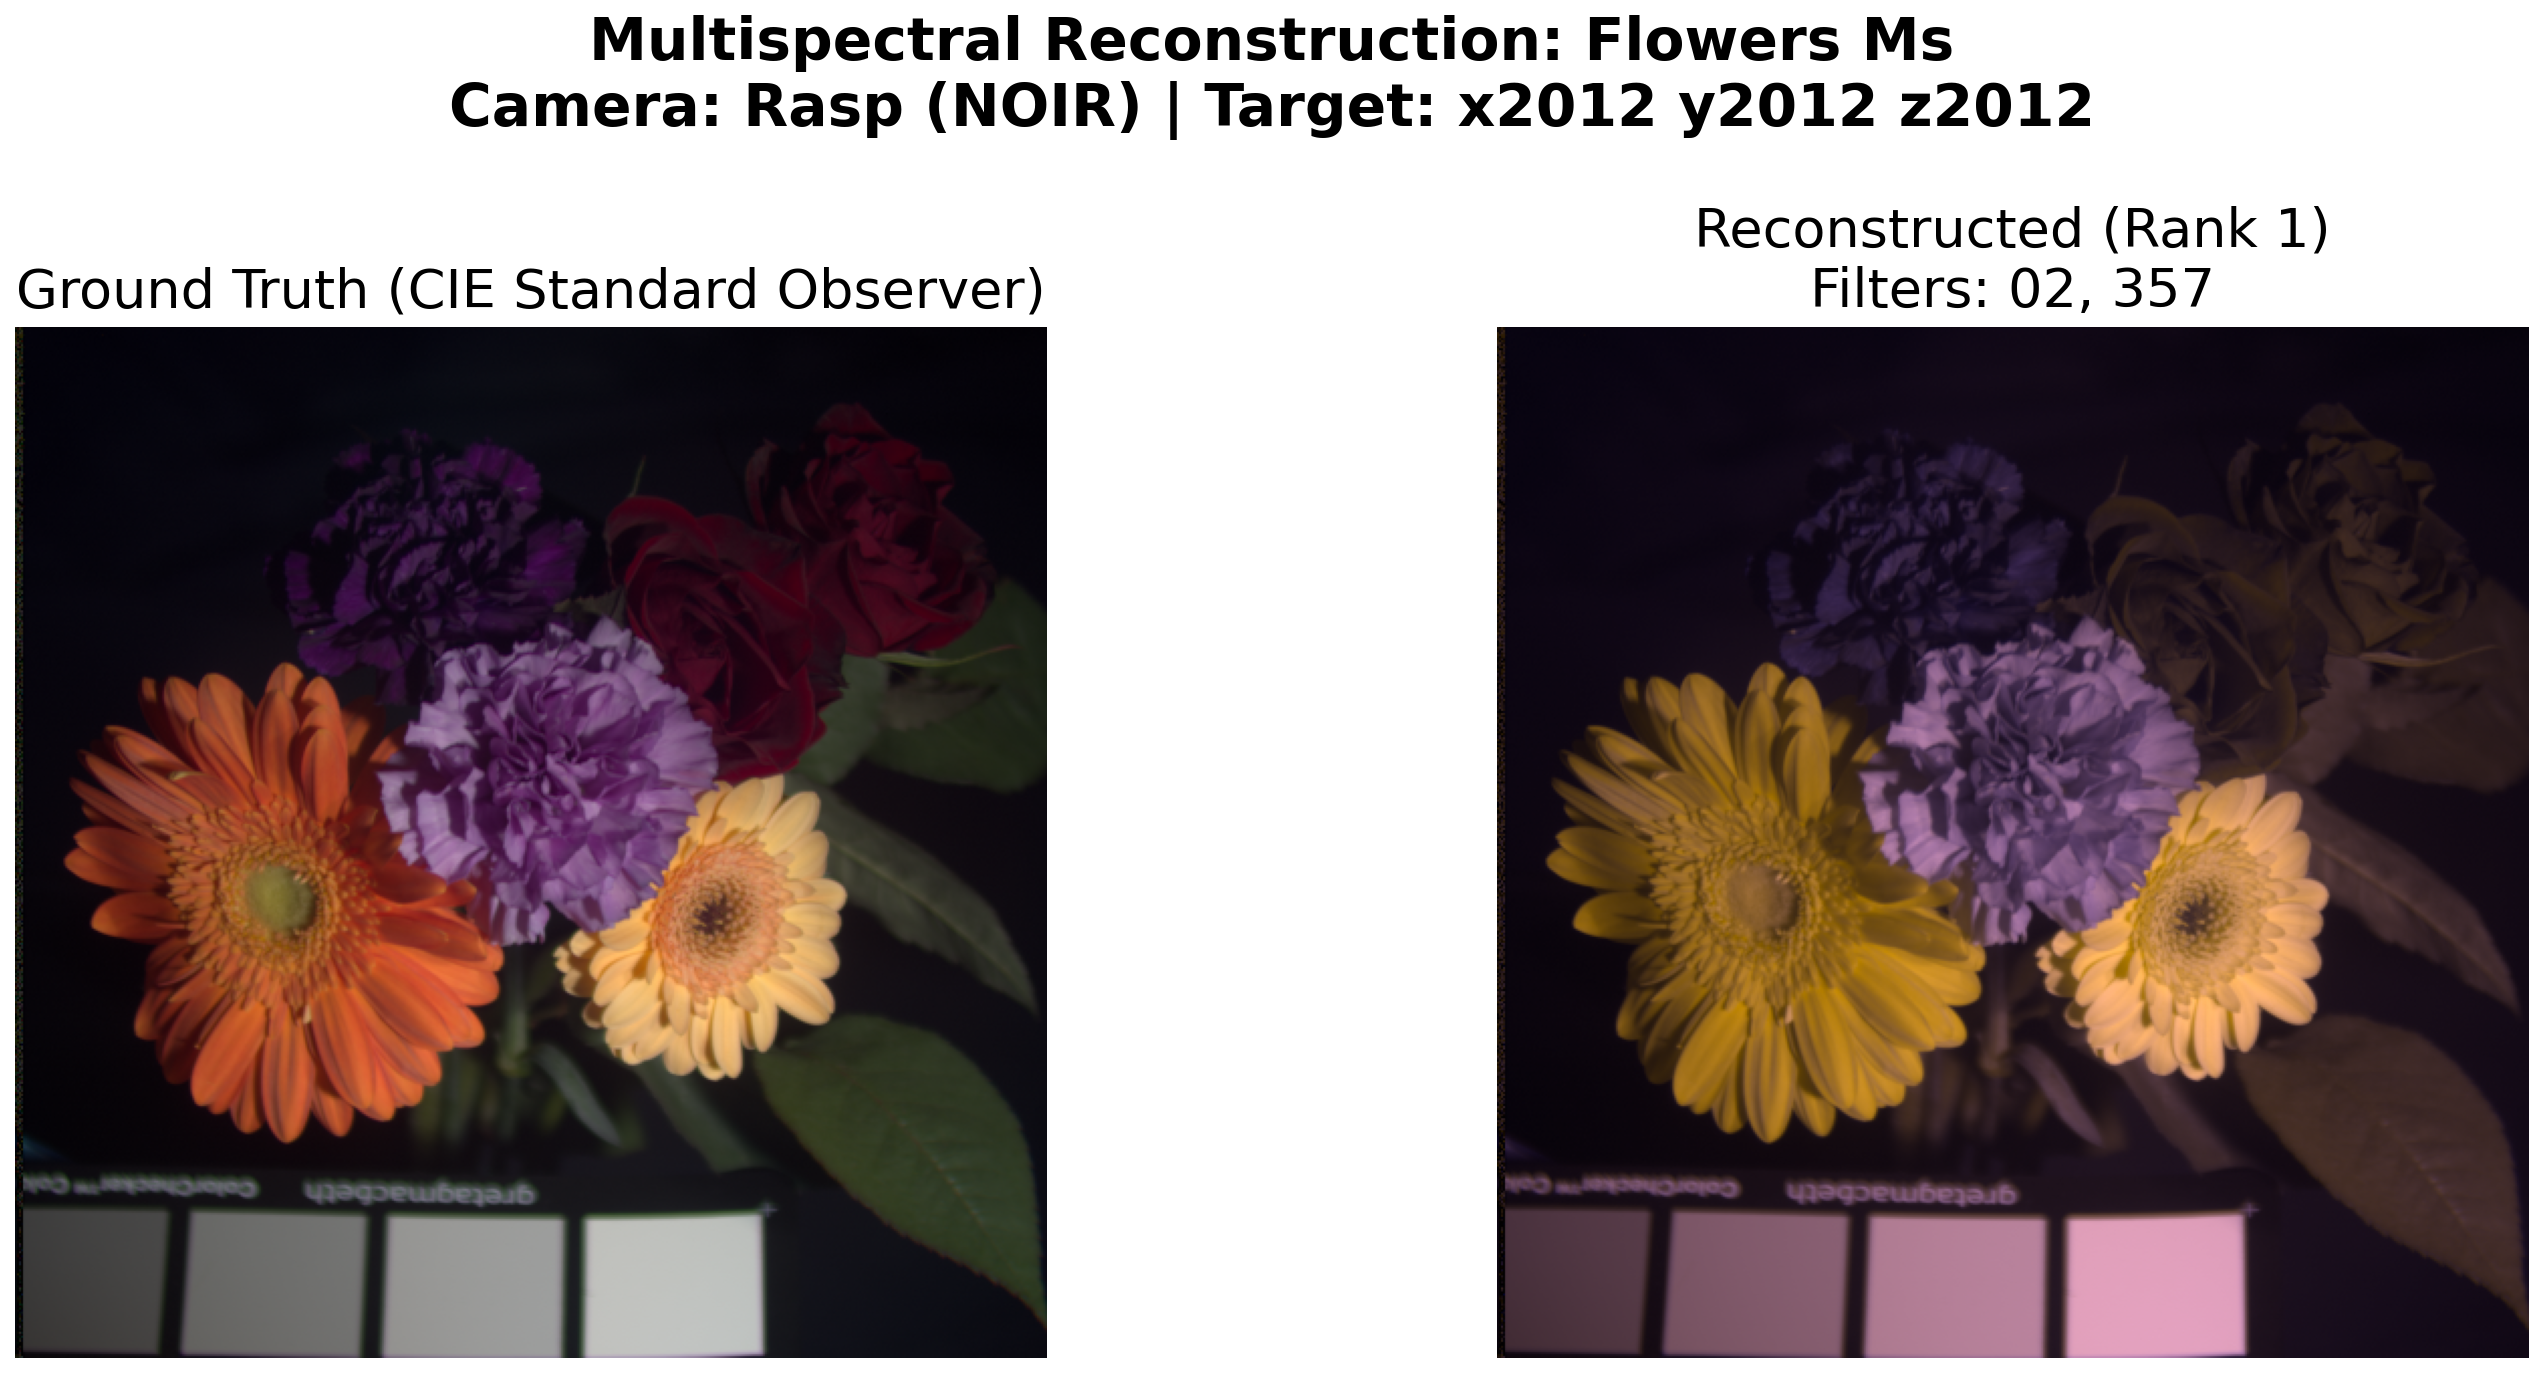
\includegraphics[width=\linewidth]{media/cave_appendix/k2flowers.png}
    \caption{$k=2$, $\dE$=13.17}
\end{subfigure}
\begin{subfigure}{.49\linewidth}
    \centering
    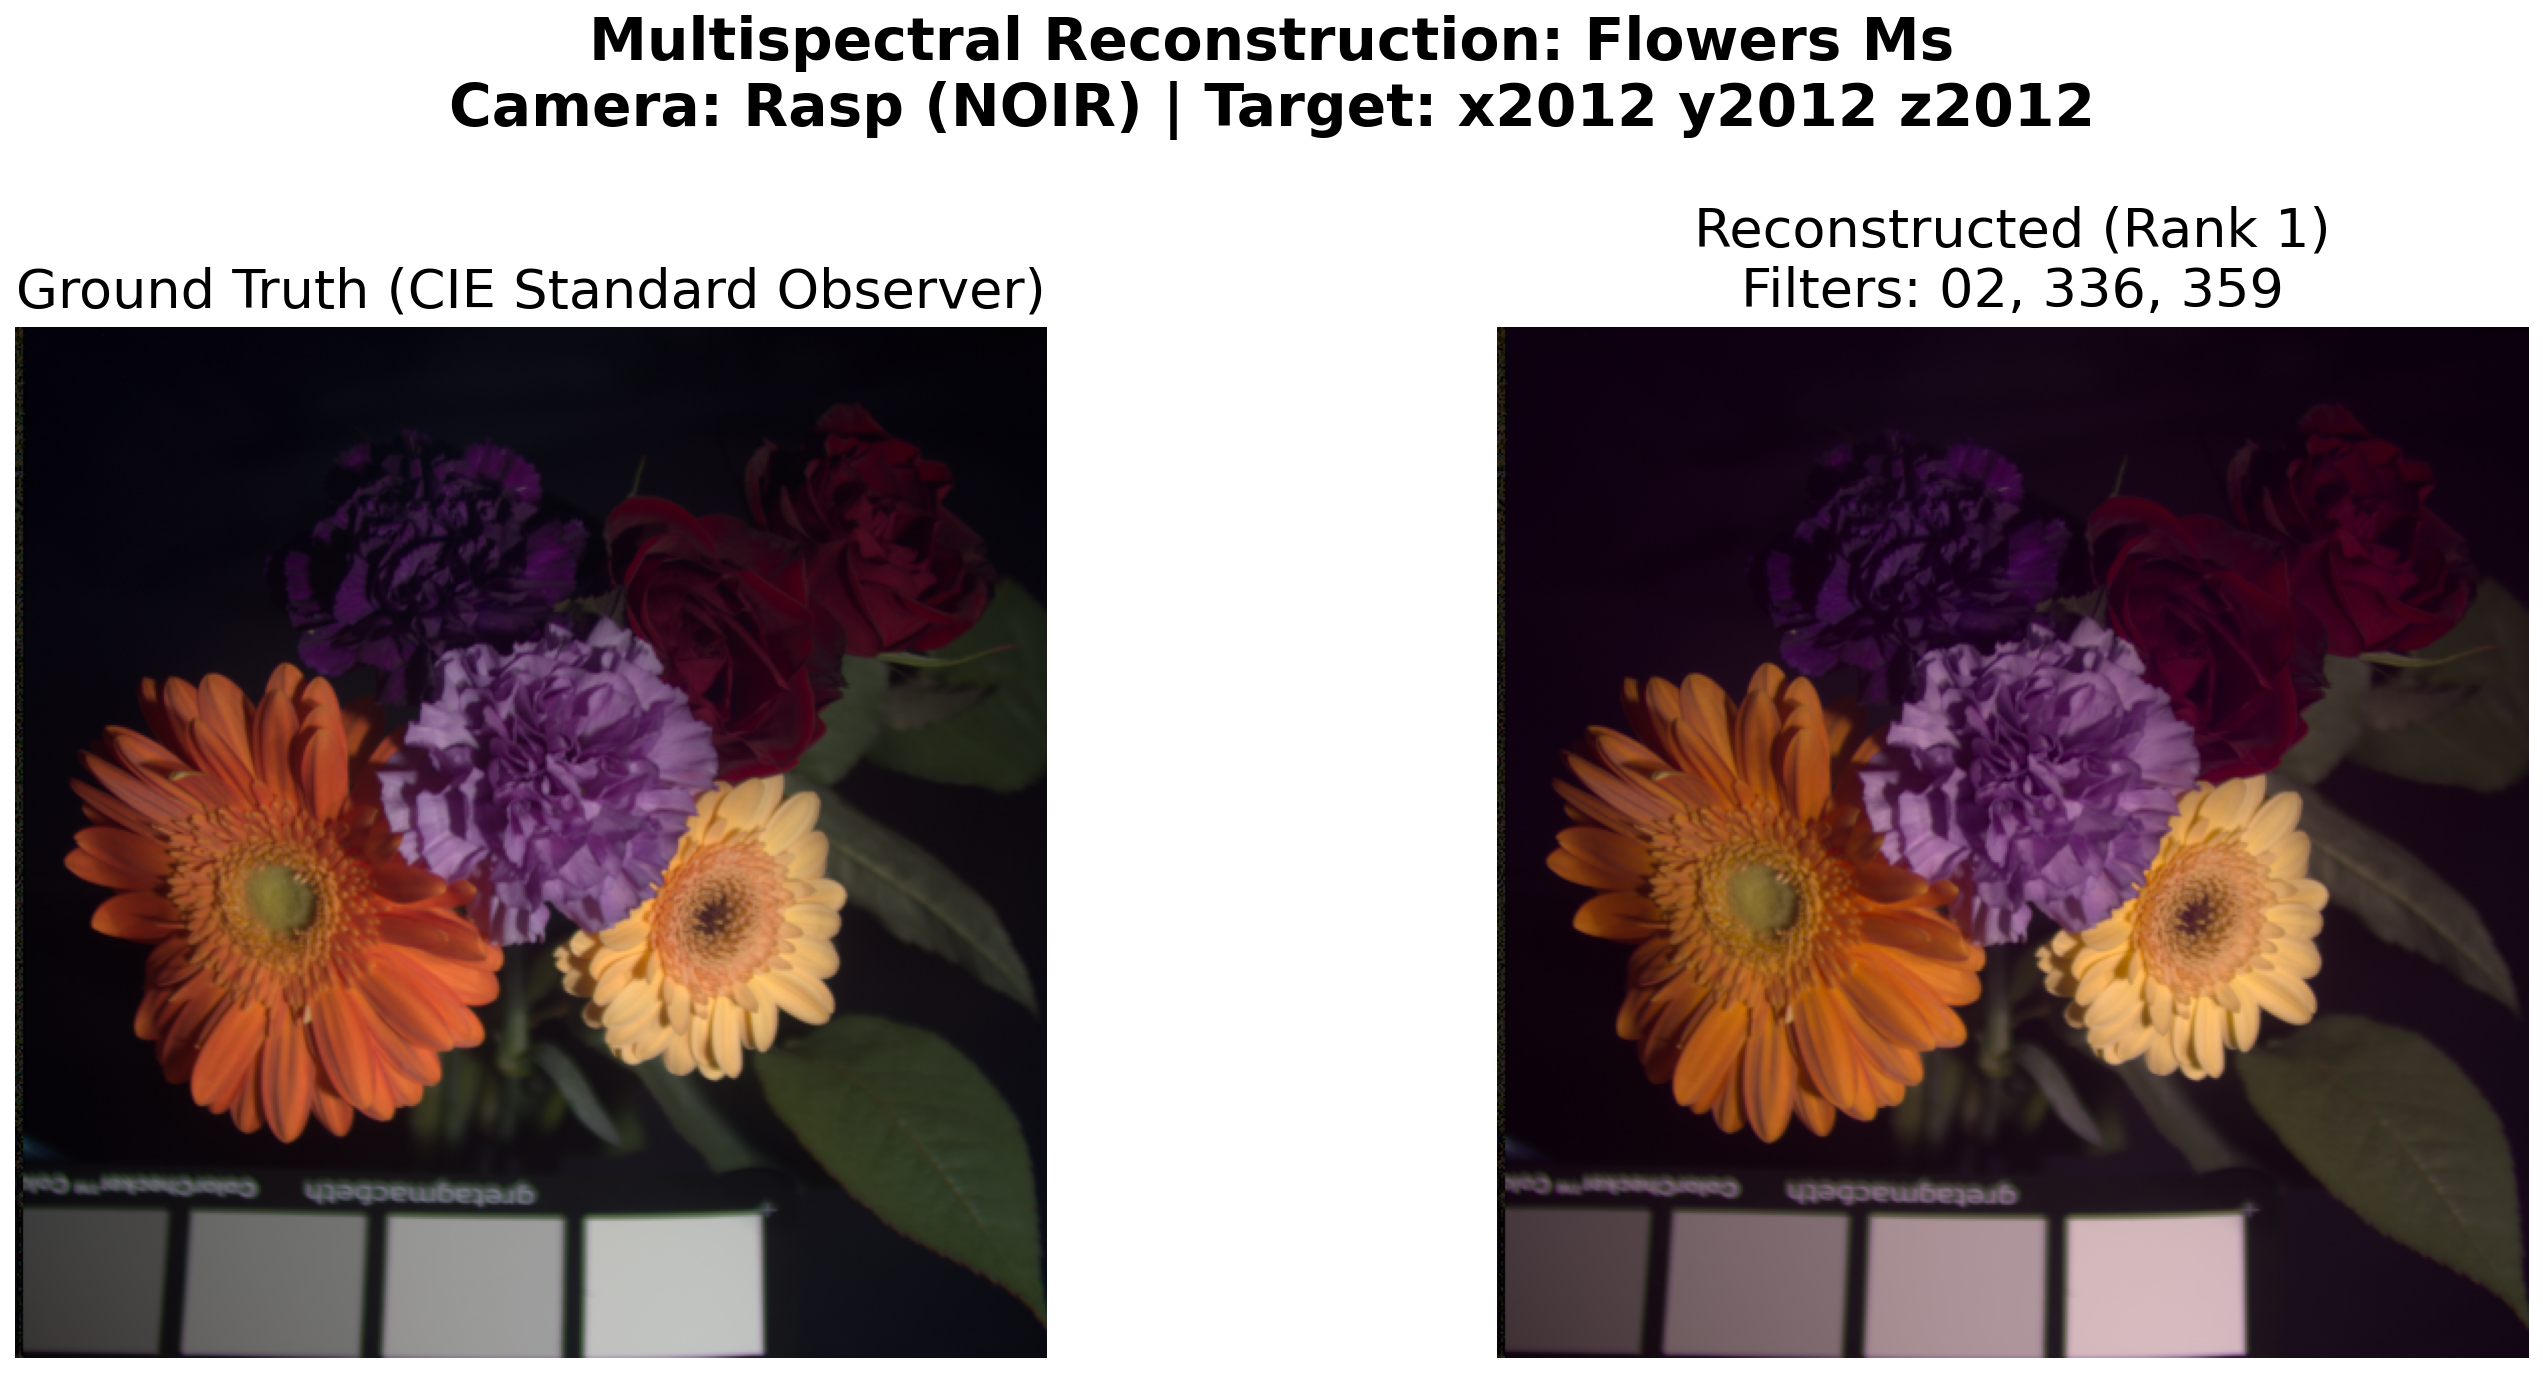
\includegraphics[width=\linewidth]{media/cave_appendix/k3flowers.png}
    \caption{$k=3$, $\dE$=5.45}
\end{subfigure}
\begin{subfigure}{.49\linewidth}
    \centering
    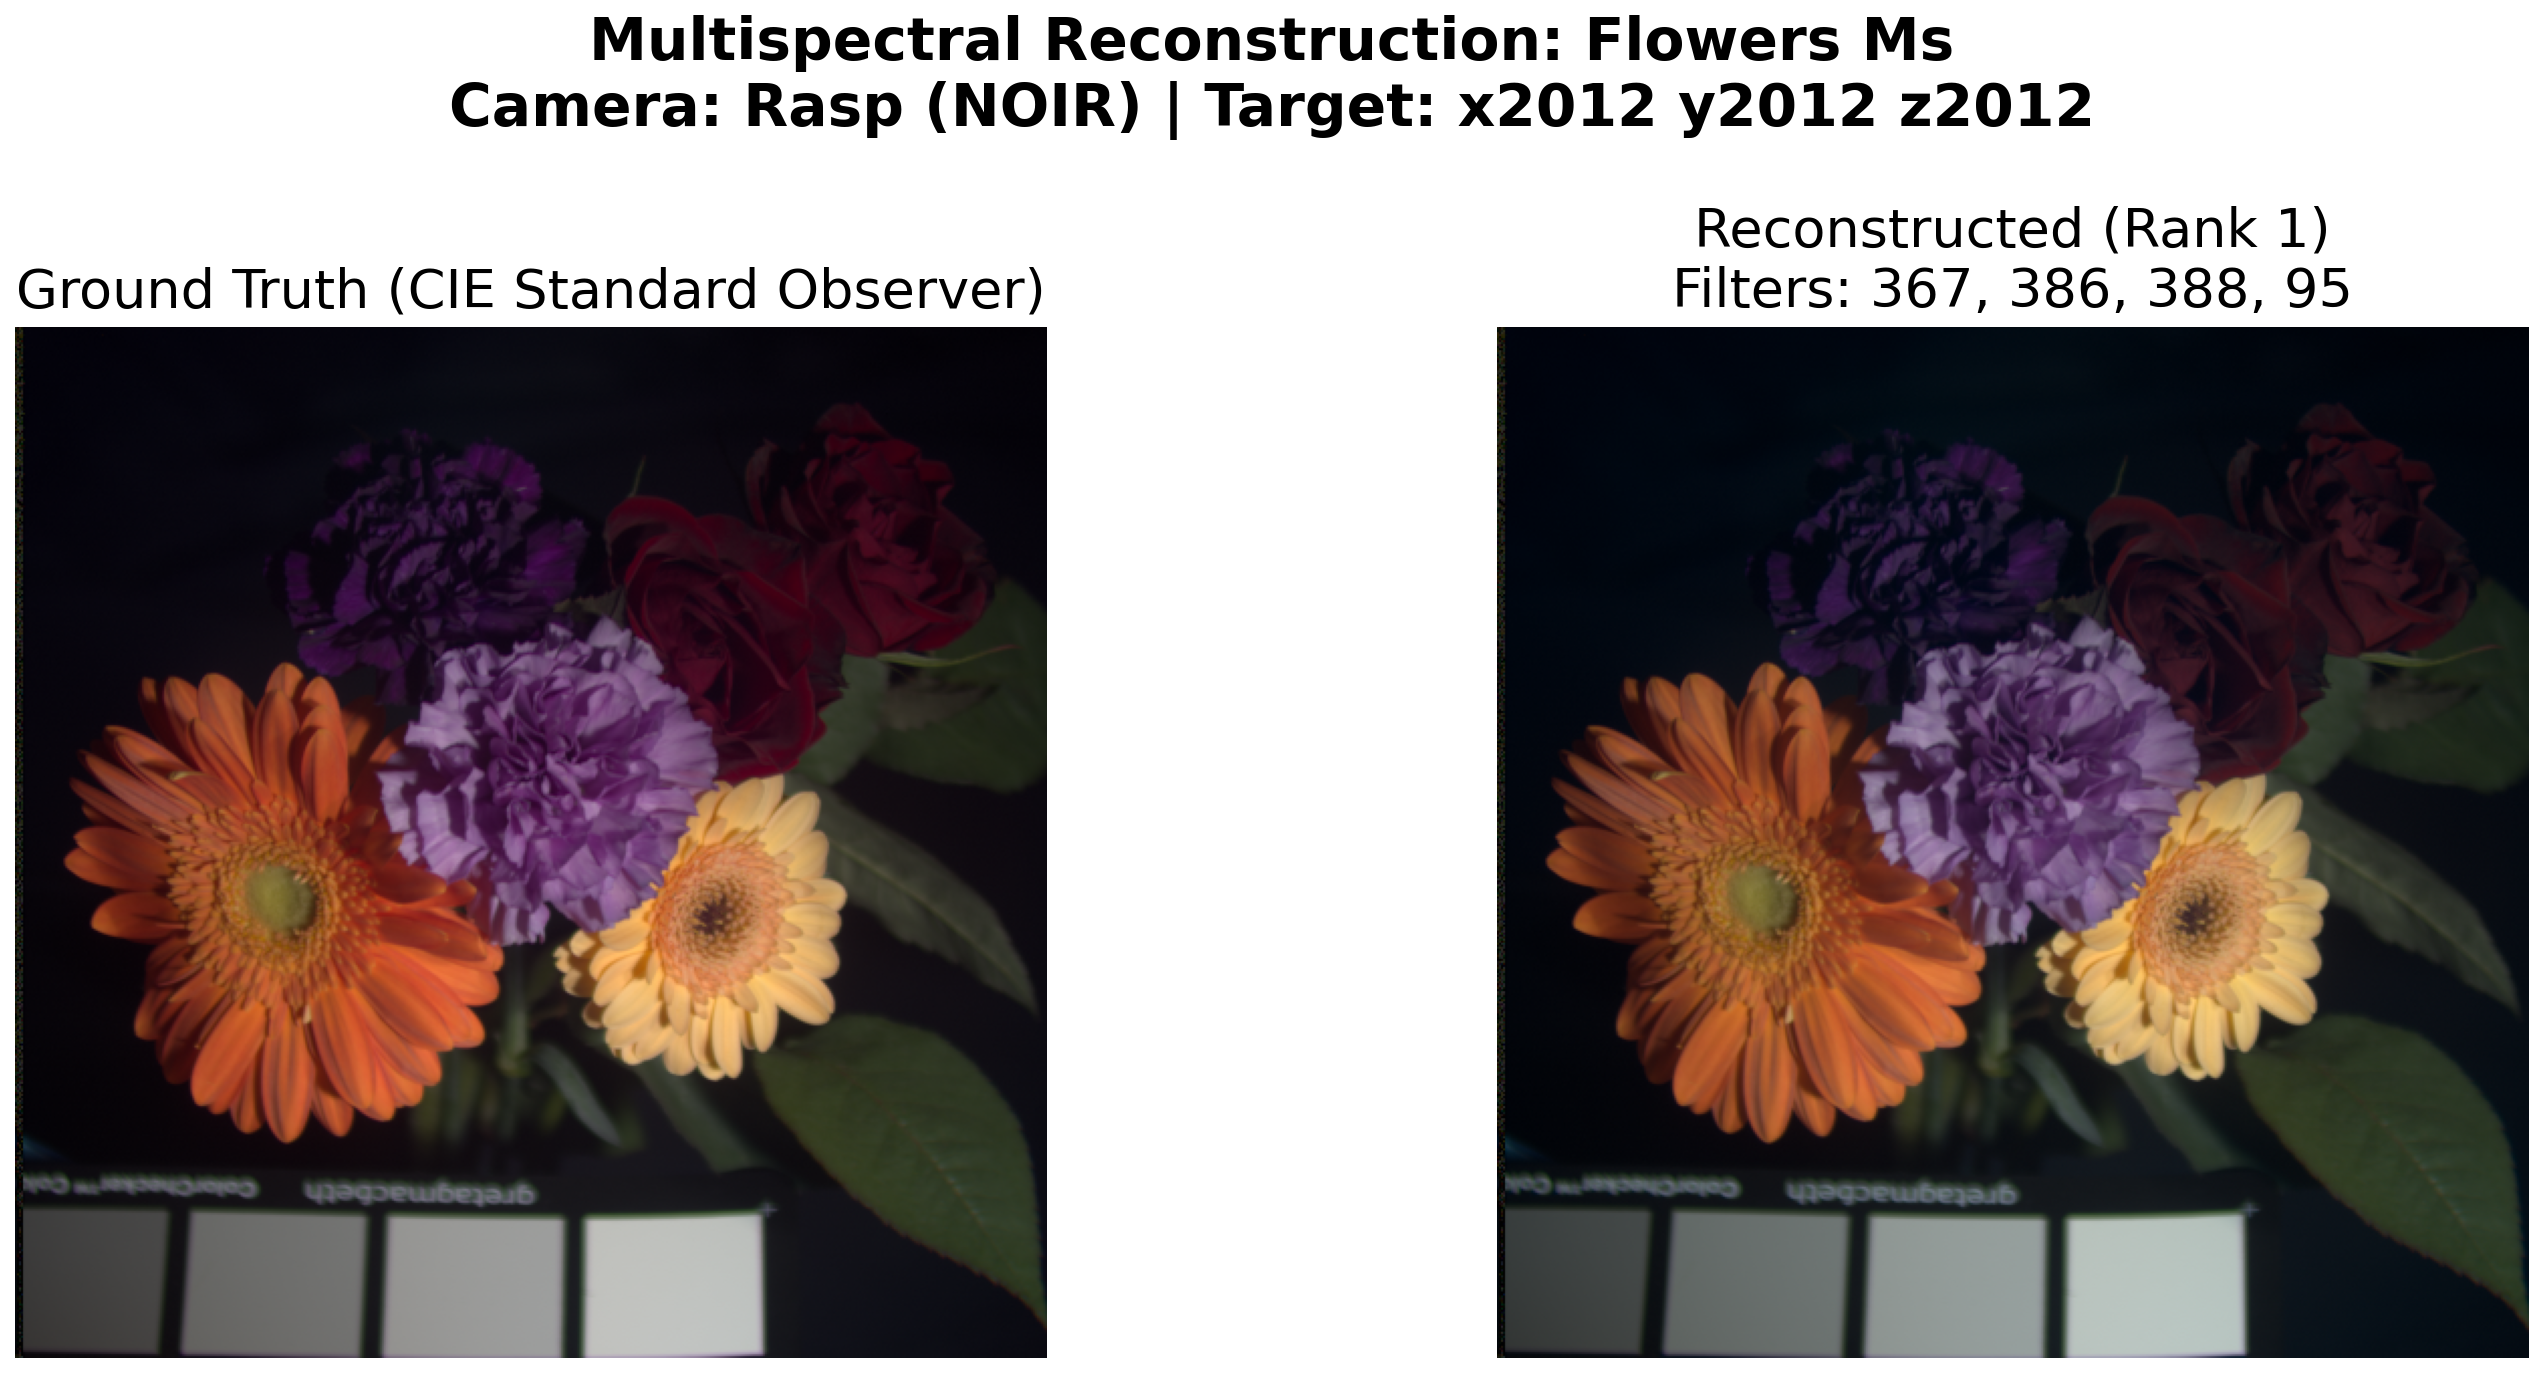
\includegraphics[width=\linewidth]{media/cave_appendix/k4flowers.png}
    \caption{$k=4$, $\dE$=1.93}
\end{subfigure}
\begin{subfigure}{.49\linewidth}
    \centering
    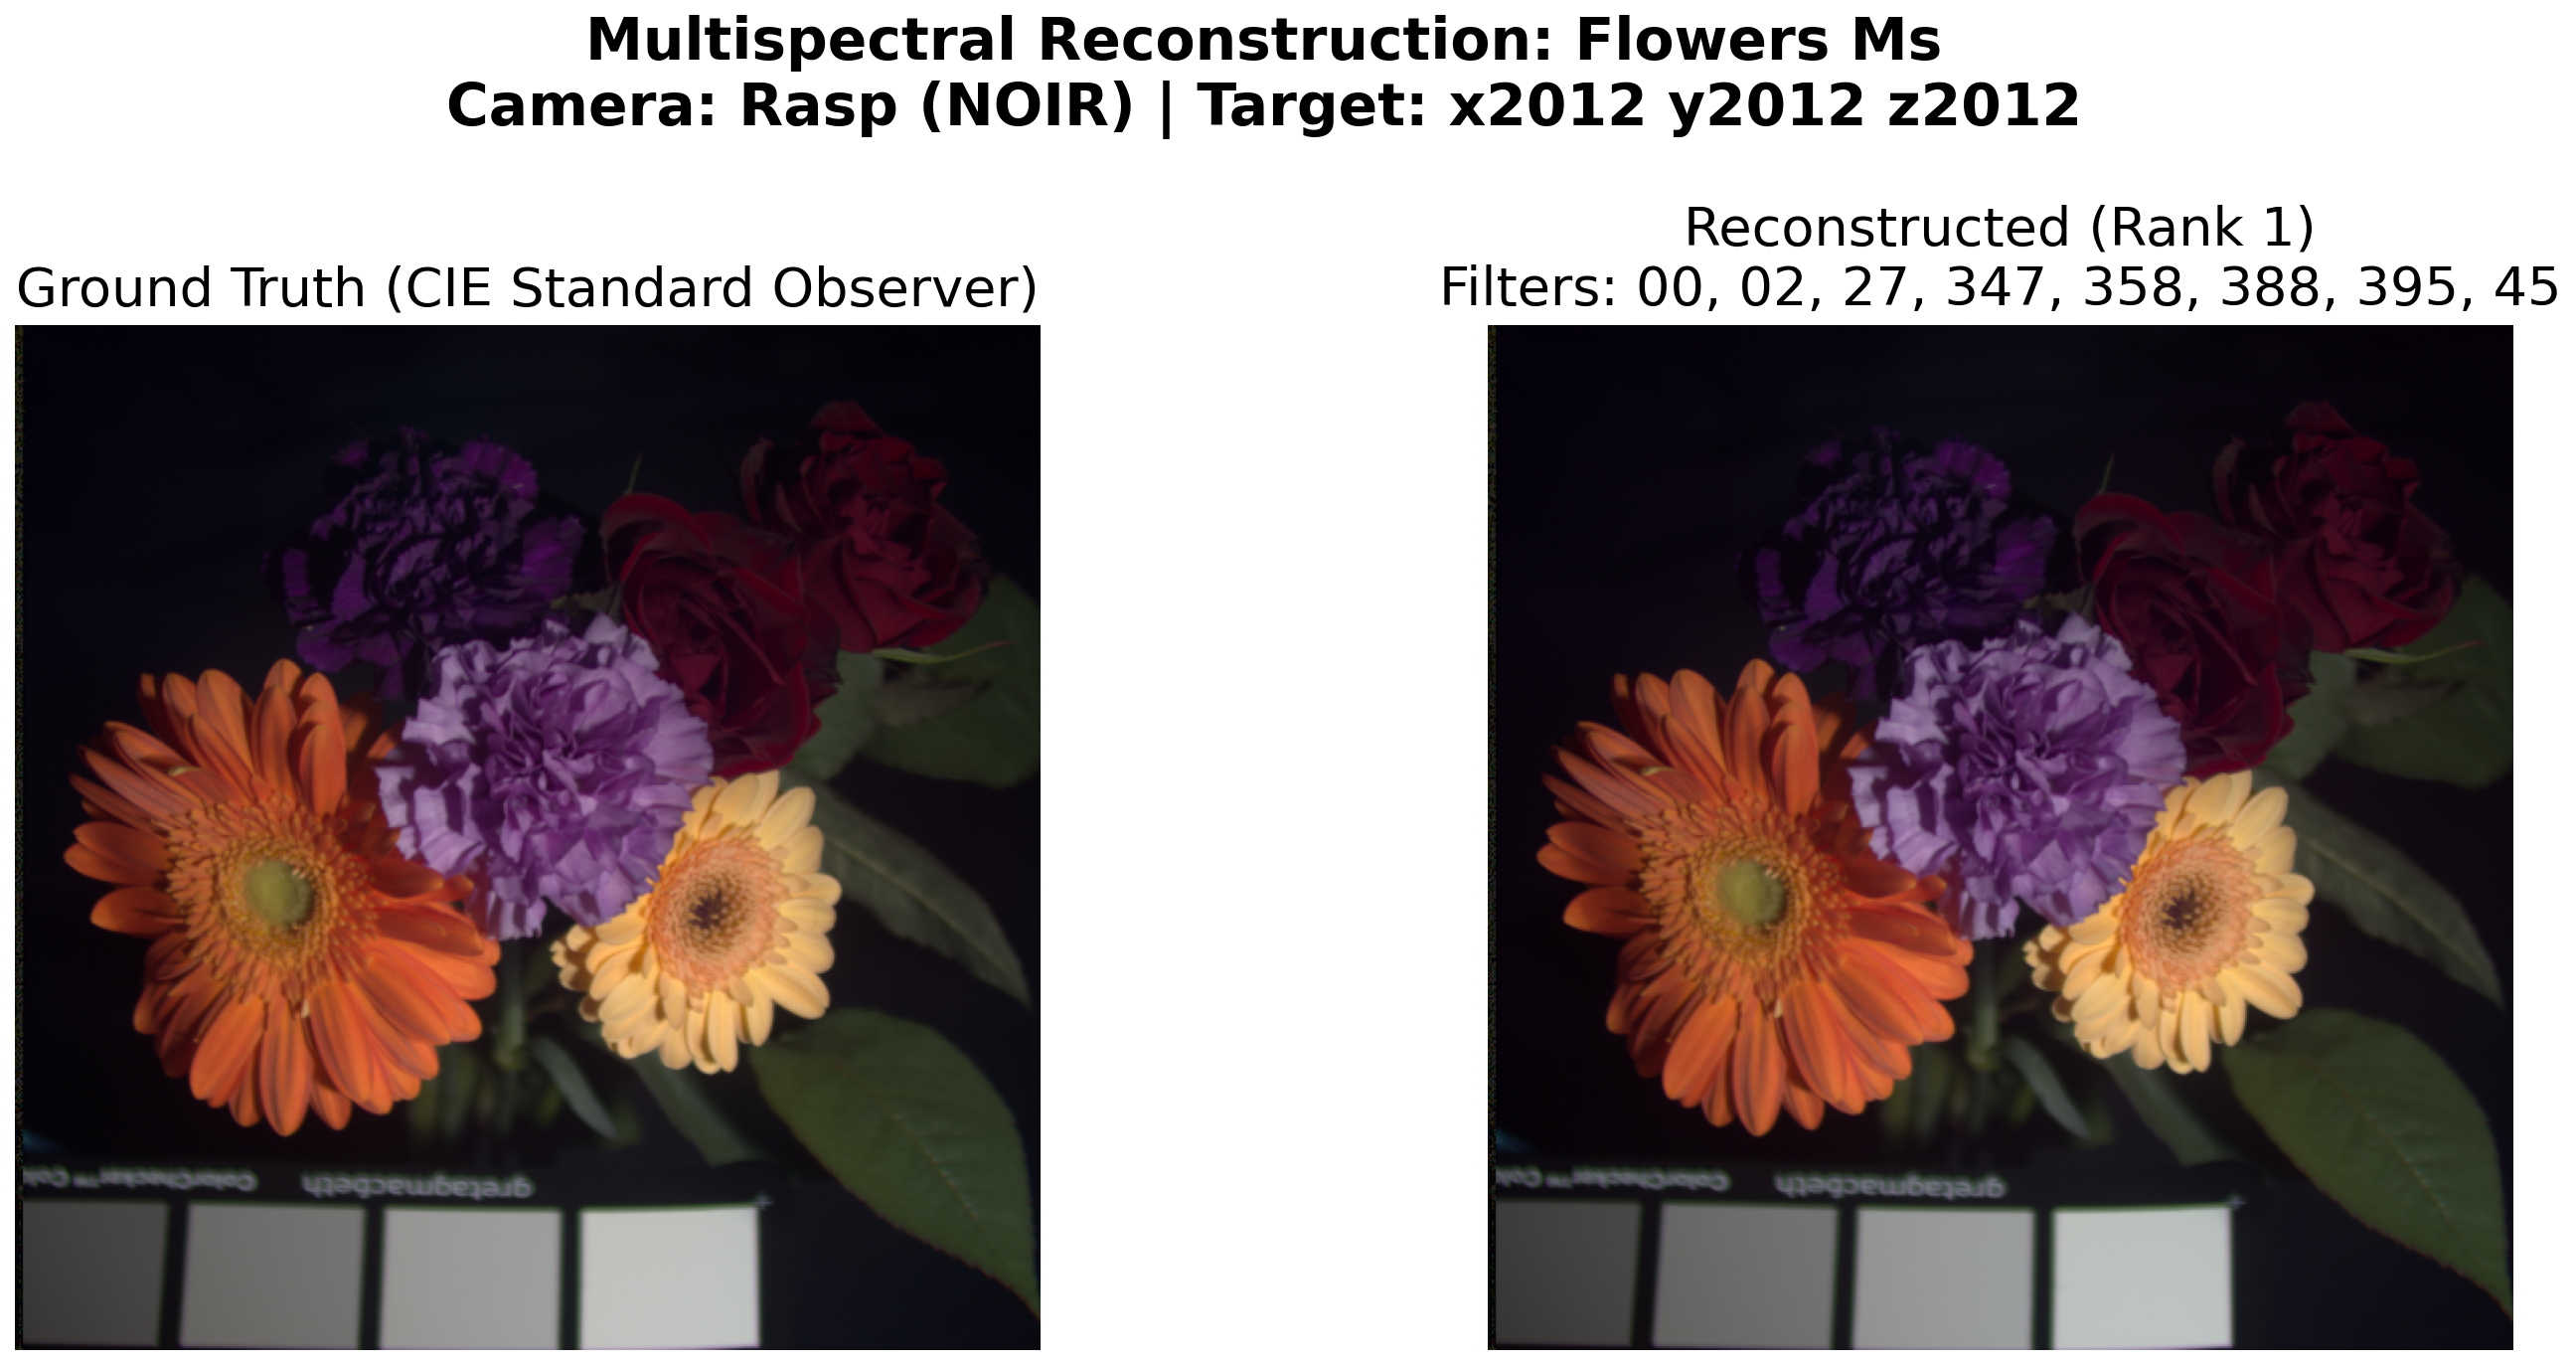
\includegraphics[width=\linewidth]{media/cave_appendix/k8flowers.png}
    \caption{$k=8$, $\dE$=.61}
\end{subfigure}
\caption{CAVE Renders of Flowers Multispectral Dataset, With Macbeth $\dE$}
\end{figure}

\subsection{Capture Errors}

A few captures in the lab featured artifacts, and a number of filters preserved transmission fairly uniformly across $\omega$ but included 'frost' or 'blur' effects which occasionally performed well in simulations but often added poor elements to reconstructions.
A number of otherwise good captures included slight lens flare near the top of the capture or just above the car, these were included as they do not affect the measurement of the PMC. 
These filters numbered $\{0, 1, 100, 101, 104, 121, 122, 124, 125, 126, 127, 160, 61, 63\}$ were excluded from the main simulation set, and another round of simulations were run with the trimmed set. 
This had negligible effect on the quality of reconstruction. 

\begin{figure}[H]
\centering
\begin{subfigure}{.49\linewidth}
    \centering
    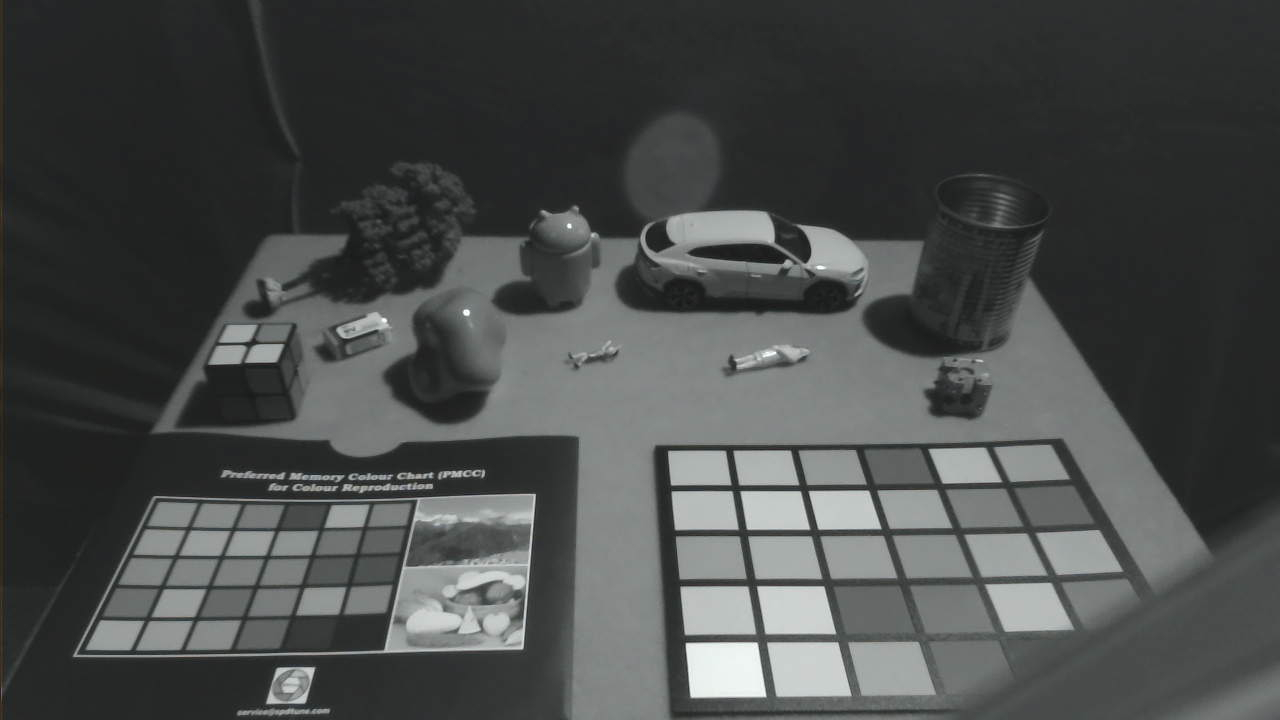
\includegraphics[width=\linewidth]{media/Lab00.jpg}
    \caption{Filter 00 in RaspberryPi Camera, excluded for artifacts in bottom right}
\end{subfigure}
\begin{subfigure}{.49\linewidth}
    \centering
    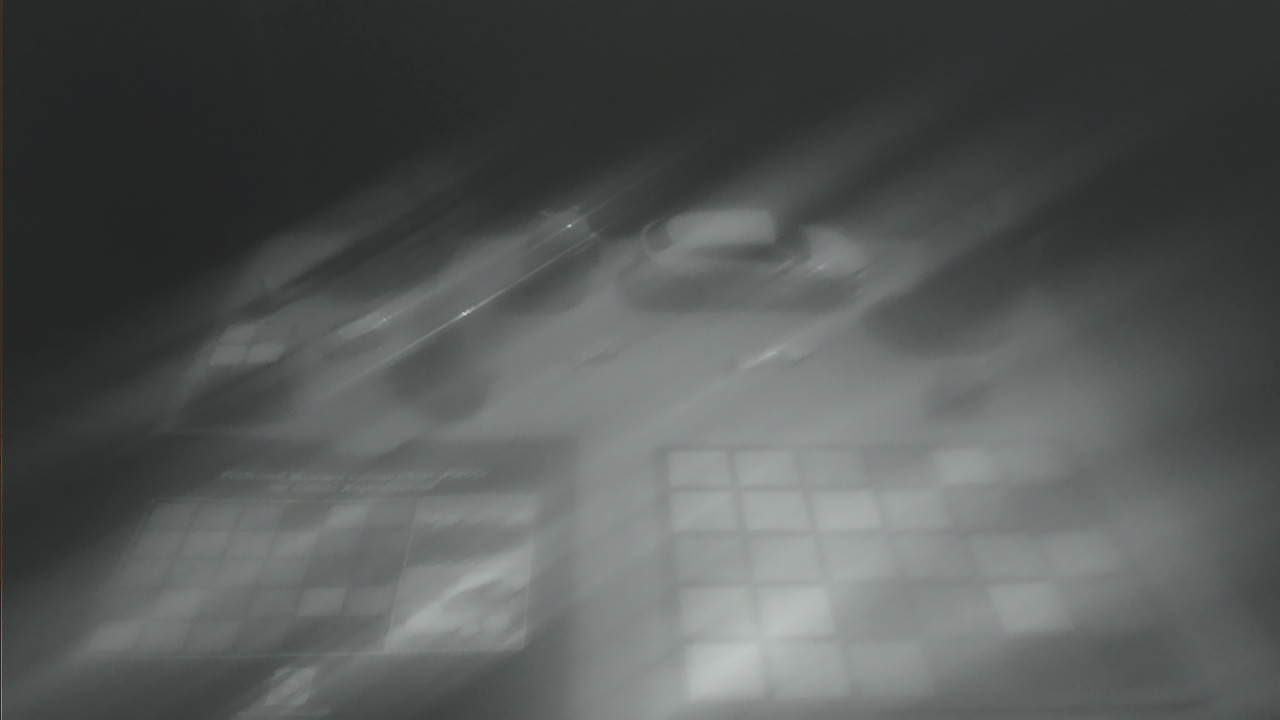
\includegraphics[width=\linewidth]{media/Lab104.jpg}
    \caption{Filter 104 in RaspberryPi Camera, excluded for blur effect}
\end{subfigure}
\begin{subfigure}{.49\linewidth}
    \centering
    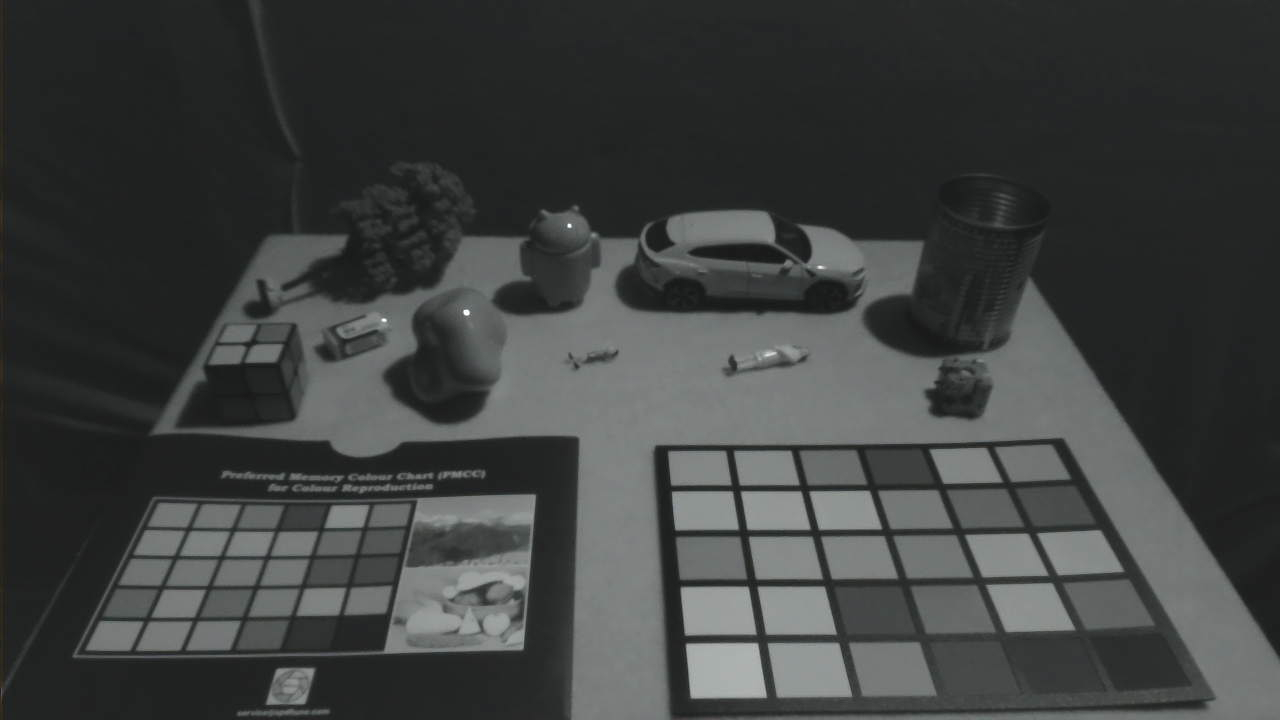
\includegraphics[width=\linewidth]{media/Lab47.jpg}
    \caption{Filter 47 in RaspberryPi Camera}
\end{subfigure}
\begin{subfigure}{.49\linewidth}
    \centering
    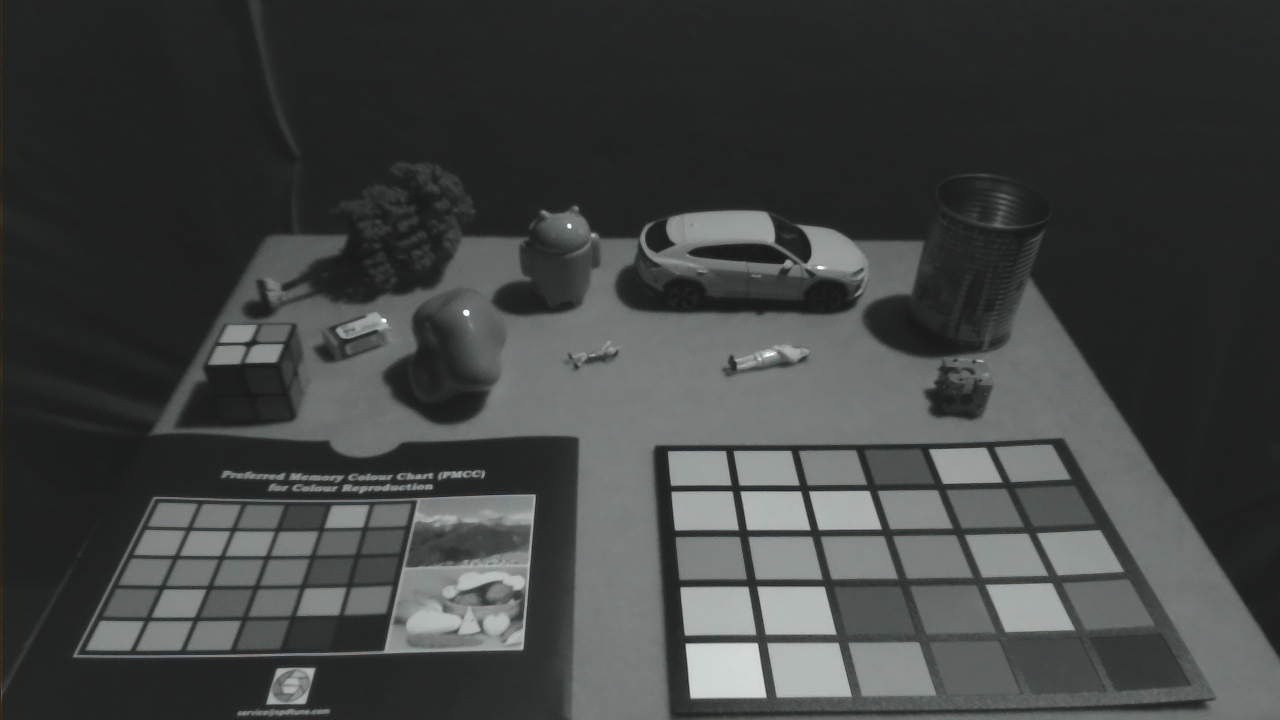
\includegraphics[width=\linewidth]{media/Lab336.jpg}
    \caption{Filter 336 in RaspberryPi Camera}
\end{subfigure}
\caption{Monochrome Captures in Lab Environment}
\end{figure}

For demonstration, we show a reconstruction for the $k=5$ case, where we simulate the optimal reconstruction including an IR-cut camera. 
However, the lab measurements were taken in the absence of an IR-cut camera, resulting in an ill-fitting reconstruction.

\begin{center}
    \centering
    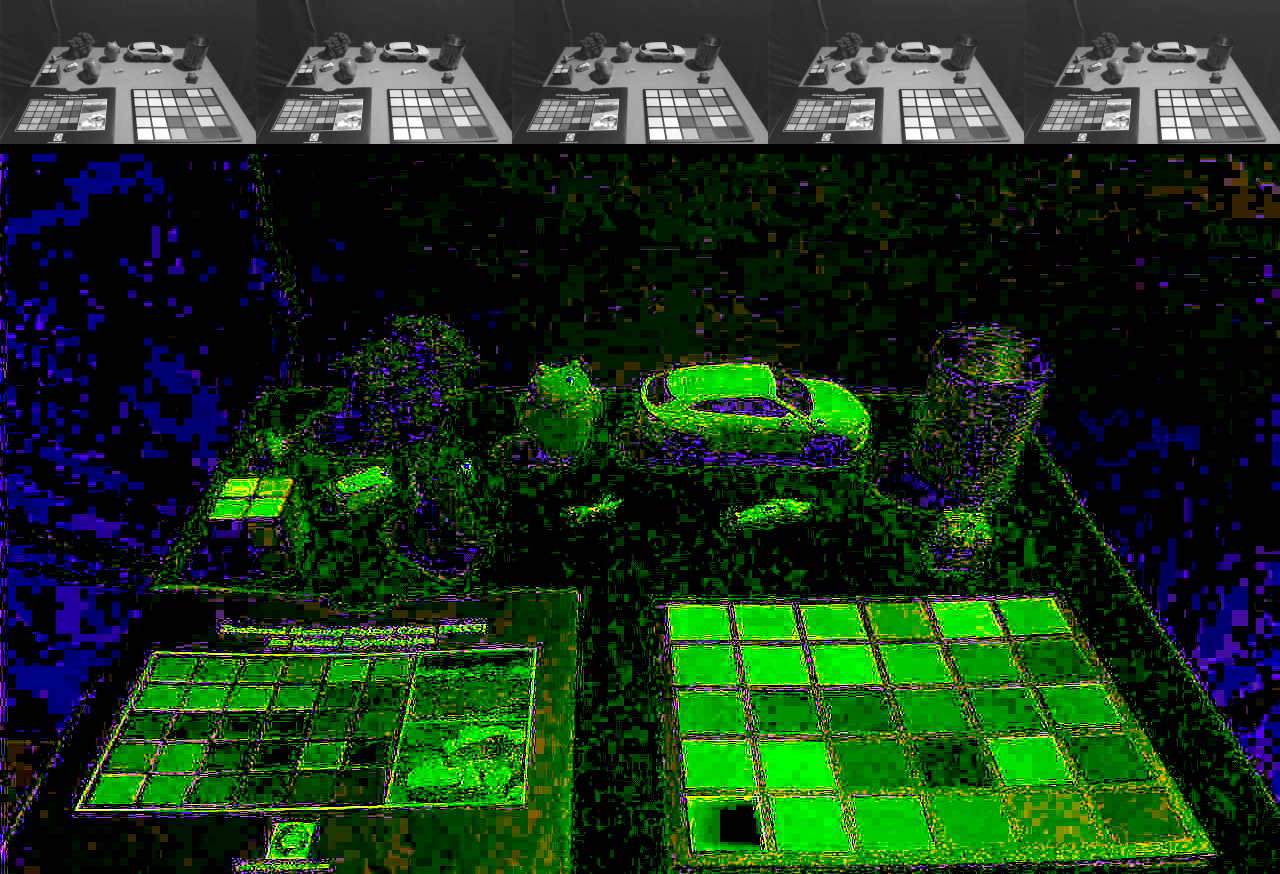
\includegraphics[width=.75\linewidth]{media/k1_5_recon_badNOIR.png}
    \captionof{figure}{$k_1=5$ Photo Lab Reconstruction with component captures above, incorrect camera configuration}
\end{center}


\subsection{In-Lab Camera Tuning}

%TODO: MOVE TO APPENDIX???
We demonstrate a poorly tuned simulation, in which we run an optimal filter selection in the presence of an IR-cut filter, but our set of captures does not include this apparatus. 
This poor example shows a different $k=5$ solution, but with the poor captures included.
Capture 00 includes a blockage in the bottom right squares in the PMC, and is therefore unfit, while filters 100 and 160 have generally poor  

\begin{figure}[H]
\centering
\begin{subfigure}{.49\linewidth}
    \centering
    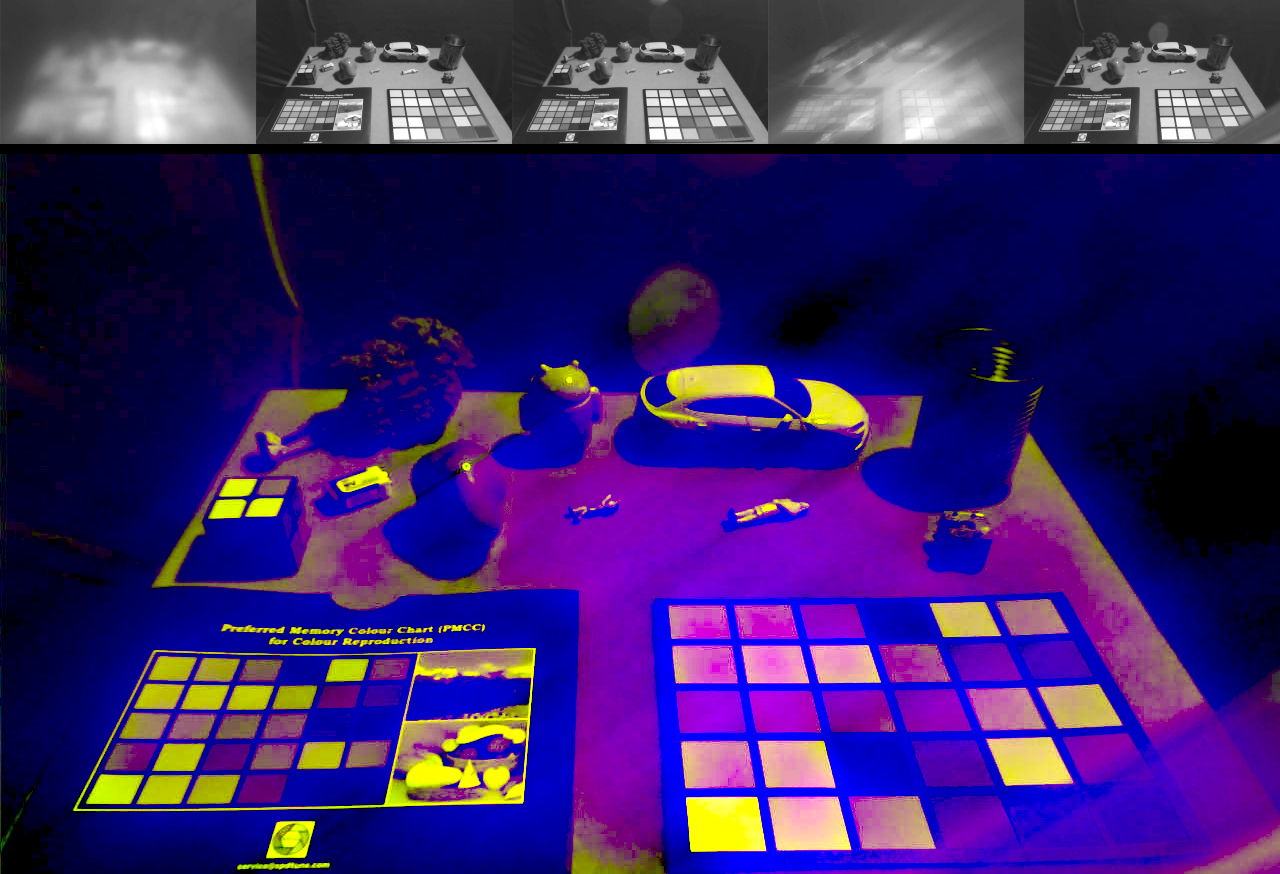
\includegraphics[width=\linewidth]{media/k5_noisy_render.png}
    \caption{Poor quality $k=5$ reconstruction including unfit filters 00, 100, 160}
\end{subfigure}
\begin{subfigure}{.49\linewidth}
    \centering
    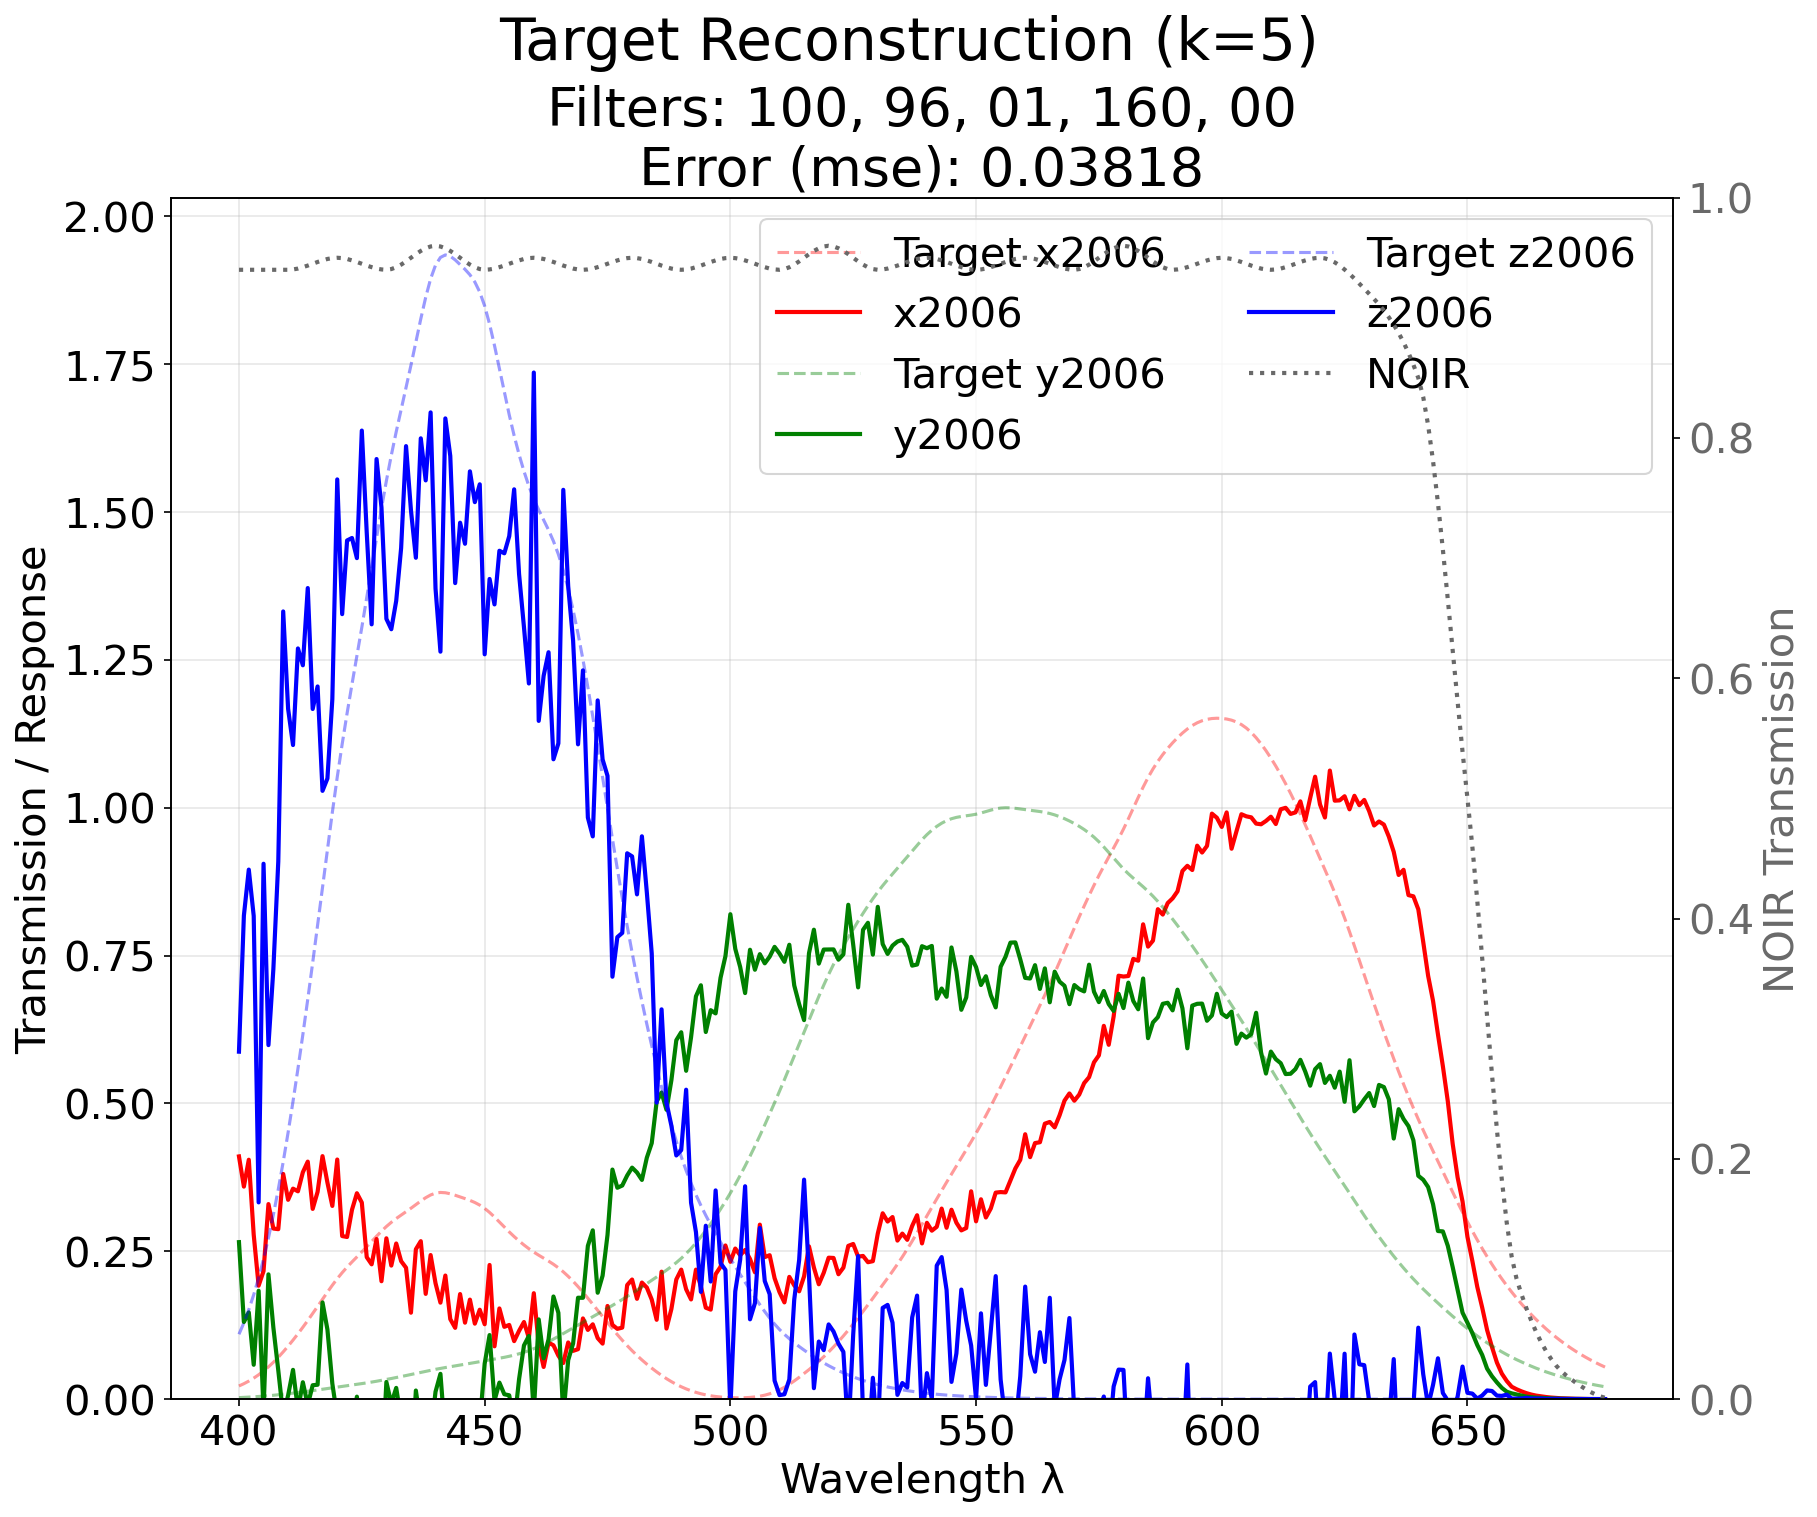
\includegraphics[width=\linewidth]{media/k5_noisy_spectra.png}
    \caption{Spectral reconstruction for $k=5$ combination with low MSE, poor realized result}
\end{subfigure}
\caption{$k=5$ filter combination with poor reconstruction quality}
\end{figure}

%TODO: if this result doesn't improve, move to appendix and explain
We also demonstrate a classical camera tuning methodology, where we minimize explicitly the average $\dE$ over the PMC. 
For $k=3$, we achieve $\dE$ of 12, which is significantly above the just-noticeable-difference threshold and warrants further investigation of potential measurement errors.
Either way, we use the simulated results for our main reconstruction efforts. 

%TODO: Improve this reconstruction
\begin{center}
    \centering
    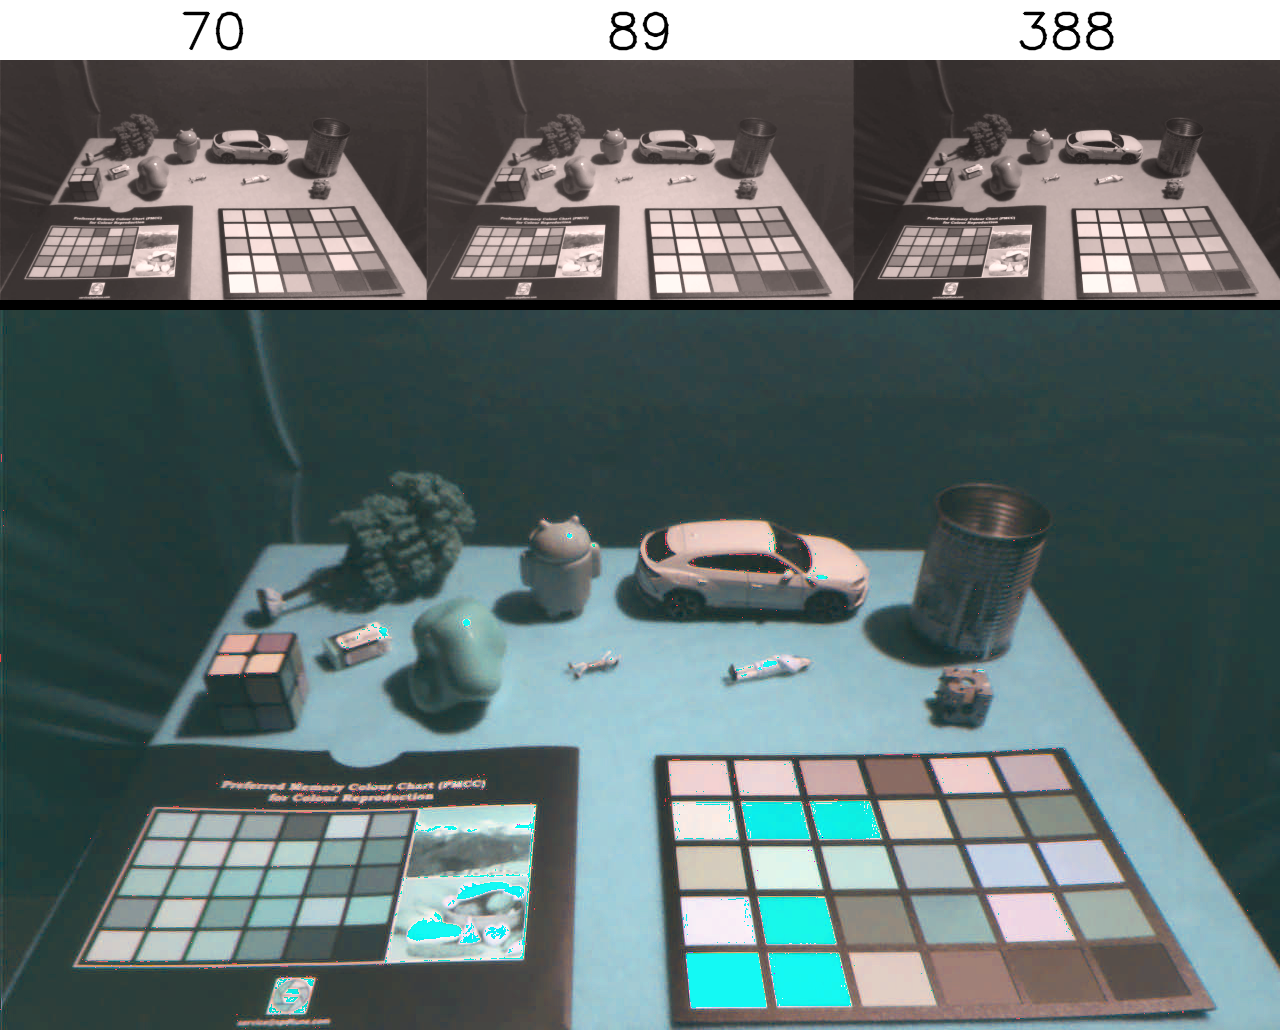
\includegraphics[width=.75\linewidth]{media/OK_recon_with_sources_70_89_388.png}
    \captionof{figure}{$k=3$ reconstruction with $\dE$ minimization}
\end{center}